% +--------------------------------------------------------------------+
% | LaTeX Template                                                     |
% | for K-State Electronic Theses, Dissertations, and Reports          |
% |                                                                    |
% | Comments and guidelines for using the template are shown           |
% | within boxes like this one.                                        |
% |                                                                    |
% | Revised 6/30/06                                                    |
% | 9/14/06: Removed typos                                             |
% +--------------------------------------------------------------------+

% +--------------------------------------------------------------------+
% | Your paper should contain the following sections, except where     |
% | indicated as optional, in the order shown.  Also, all headings     |
% | shown with an asterisk (*) must be centered and in uppercase       |
% | letters:                                                           |
% |                                                                    |
% | Abstract Title Page (doctoral dissertations only)                  |
% | ABSTRACT* (doctoral dissertations only)                            |
% | Title Page                                                         |
% | Copyright Page (Optional - only needed if copyrighting)            |
% | ABSTRACT *                                                         |
% | TABLE OF CONTENTS *                                                |
% | LIST OF FIGURES *                                                  |
% | LIST OF TABLES*                                                    |
% | ACKNOWLEDGMENTS* (Optional)                                        |
% | DEDICATION * (Optional)                                            |
% | PREFACE * (Optional)                                               |
% | Individual Chapters                                                |
% | References and/or bibliography                                     |
% | Appendices (as needed)                                             |
% +--------------------------------------------------------------------+

% +--------------------------------------------------------------------+
% | The LaTex keyword \documentclass selects a particular class to     |
% | associate with the document.  The current documentclass            |
% | {class_diss} generates a Table of Contents that has leading dots   |
% | only on chapter subheadings.  If you prefer a Table of Contents    |
% | that has leading dots for all entries, replace {class_diss}        |
% | with {Mydiss} in the command below.                                |
% |                                                                    |
% +--------------------------------------------------------------------+

\documentclass[final, 12pt, oneside]{class_diss}
%\documentclass[final, 12pt, twoside, openright]{class_diss}

% +--------------------------------------------------------------------+
% | The following command sets the bibliography style to American
% | Institute of Physics (AIP).  Other styles are available in the
% | styles directory.  To use a different style, replace "aip" with
% | the filename of the style you want to use.
% +--------------------------------------------------------------------+

%\bibliographystyle{styles/plain}

\usepackage[utf8]{inputenc}
\usepackage[T1]{fontenc}
\usepackage[spanish,es-tabla]{babel}
\selectlanguage{spanish}
\usepackage{eurosym}
\usepackage{xspace}
\usepackage[usenames,dvipsnames,svgnames,table]{xcolor}
\usepackage{graphicx}
\usepackage{booktabs}

% +--------------------------------------------------------------------+
% | Now, we add in all external packages that we will use throughout   |
% | the document.  You can add other packages as needed.
% +--------------------------------------------------------------------+

%\usepackage{     caption2} % Customize captions a bit more
\usepackage{      amsmath} % American Mathematics Society standards
%\usepackage{      wrapfig} % Wraps text around a figure or table
\usepackage{     graphicx} % Extended graphics package.
%\usepackage{     fancyhdr} % Efficiently handles headers and footers
%\usepackage{       braket} % Bra-Ket notation package
%\usepackage{     mathrsfs} % Specialized Math fonts (Hamiltonian, etc.)
%\usepackage{boxedminipage} % Boxed text can be produced
%\usepackage{     setspace} % Controls line spacing via \begin{space}

\usepackage{amsxtra}
\usepackage{amssymb}
\usepackage{amsthm}
\usepackage{latexsym}

\usepackage{enumerate}
\usepackage{float}

%% Paquetes propios
\usepackage{subcaption}
\usepackage{framed}
\usepackage{listings}

\lstset{language=C++,
  basicstyle=\footnotesize\ttfamily,
  keywordstyle=\color{blue}\ttfamily,
  stringstyle=\color{red}\ttfamily,
  commentstyle=\color{green}\ttfamily,
  morecomment=[l][\color{magenta}]{\#},
  xleftmargin=2em,
%  frame=single,
  frame=lines,
  framexleftmargin=0em,
  numbers=left,
  escapechar=|
}

% +--------------------------------------------------------------------+
% | The color package allows one to select colors for hyperlinking     |
% | (see below).                                                       |
% +--------------------------------------------------------------------+

%\usepackage[usenames]{color}

% +--------------------------------------------------------------------+
% | Colors defined for use with this template.                         |
% +--------------------------------------------------------------------+

\definecolor{  Pink}{rgb}{1.0, 0.5, 0.5}
\definecolor{Maroon}{rgb}{0.8, 0.0, 0.0}

% +--------------------------------------------------------------------+
% | In the commands below, we use the 'natbib' package, and specify    |
% | the 'sort&compress' option, which condenses                        |
% | citations from (1,2,3,5,9,10,11) to (1-3,5,9-11).  The 'bibpunct'  |
% | option selects various parameters for how the citation will be     |
% | displayed.  In this case, only the comma (separation between       |
% | citations) and the 's' (superscript) arguments are chosen.  The    |
% | other curly braces deal with how to 'wrap' the citation (using     |
% | parentheses, brackets, etc.) and are not needed for the chosen     |
% | style.                                                             |
% +--------------------------------------------------------------------+

\usepackage[sort&compress]{natbib}
%\bibpunct{}{}{,}{s}{}{}
%\usepackage{hypernat}

% +--------------------------------------------------------------------+
% | Lastly, the hyperref package allows one to hyperlink cross-        |
% | references and figures in a LaTeX document.                        |
% +--------------------------------------------------------------------+

\usepackage[pdftex, plainpages=false, pdfpagelabels]{hyperref}
\usepackage{url}

\hypersetup{
    linktocpage=true,
    colorlinks=true,
    bookmarks=true,
    citecolor=blue,
    urlcolor=red,
    linkcolor=Maroon,
    citebordercolor={1 0 0},
    urlbordercolor={1 0 0},
    linkbordercolor={.7 .8 .8},
    breaklinks=true,
    pdfpagelabels=true,
    }

% +--------------------------------------------------------------------+
% | Page margins are set on 1 inch on all sides.                       |
% +--------------------------------------------------------------------+

\topmargin      = -0.56in
\textheight     =  8.60in
\textwidth      =  6.46in
\oddsidemargin  =  0.02in



% +--------------------------------------------------------------------+
% | Comandos propios para facilitar la revision                        |
% +--------------------------------------------------------------------+
%% DEFINICIONES
\usepackage{tikz}

\let\oldmarginpar\marginpar
\renewcommand{\marginpar}[3][rectangle,draw,fill=orange,rounded corners]{%
  \oldmarginpar{%
    \tikz \node at (0,0) [#1]{#2};
  #3}%
}

\newcommand{\todo}[1]{{\color{red} \textbf{TODO: }#1 }}
\newcommand{\Todo}[1]{{\large \color{red} \textbf{TODO: }#1 }}
\newcommand{\comentario}[1]{\marginpar{Comentario}{#1}{}}
\newcommand{\rev}[1]{{\color{green}#1}}

%%%%%%%%%%%%%%%%%%%%  MACROS  %%%%%%%%%%%%%%%%%%%%%%%%%%%%%%%%%%%%%%%%%%
%\input{macros}
\newcommand{\wt}{{\em worker thread}\xspace}
\newcommand{\wts}{{\em worker threads}\xspace}
\newcommand{\odroid}{{\sc Odroid}\xspace}
\newcommand{\juno}{{\sc Juno}\xspace}
\newcommand{\gemm}{{\sc gemm}\xspace}
\newcommand{\syrk}{{\sc syrk}\xspace}
\newcommand{\trsm}{{\sc trsm}\xspace}
\newcommand{\potrf}{{\sc potrf}\xspace}
\newcommand{\Jc}{{\cal J}_c}
\newcommand{\Pc}{{\cal P}_c}
\newcommand{\Ic}{{\cal I}_c}

\newcommand{\ompss}{OmpSs\xspace}
\newcommand{\nanos}{{\sc Nanos++}\xspace}
%%%%%%%%%%%%%%%%%%%%  END MACROS  %%%%%%%%%%%%%%%%%%%%%%%%%%%%%%%%%%%%%%%%%%



% +--------------------------------------------------------------------+
% | The document finally begins here.                                  |
% +--------------------------------------------------------------------+

\begin{document}


  \setcounter{page}{-1}


% +--------------------------------------------------------------------+
% | Title Page -- Required for both Doctoral and Masters Students
% +--------------------------------------------------------------------+

% +--------------------------------------------------------------------+
% | Title Page
% +--------------------------------------------------------------------+

\newpage

% +--------------------------------------------------------------------+
% | This page should not contain a page number.  We use the
% | \thispagestyle[empty] command below to suppress page numbers
% | and other style elements.
% +--------------------------------------------------------------------+

\thispagestyle{empty}

% +--------------------------------------------------------------------+
% | The Title page begins here.
% +--------------------------------------------------------------------+

\begin{center}

   \vspace{1cm}

% +--------------------------------------------------------------------+
% | On the line below, replace "ENTER YOUR TITLE" with the title of
% | your ETDR.  Use all CAPITAL LETTERS.
% +--------------------------------------------------------------------+

   {\Large Evaluación y optimización de rendimiento y consumo energético de aplicaciones
	paralelas a nivel de tareas sobre arquitecturas asimétricas}\\

   \vspace{0.5cm}



   \vspace{0.5cm}



   {\large Costero Valero, Luis María}\\

   \vspace{0.5cm}

   MÁSTER EN INGENIERÍA INFORMÁTICA. FACULTAD DE INFORMÁTICA\\ 
   UNIVERSIDAD COMPLUTENSE DE MADRID \\

   \vspace{0.65cm}
   \rule{2in}{0.5pt}\\
   \vspace{0.85cm}

  
\includegraphics[height=2.5in]{Figures/escudo.jpg}
  

%+-- Escribe el nombre de tu asignatura de fin de master (Ingeniería de computadores,....)
   \vspace{0.5cm}
Trabajo Fin de Máster 

   \vspace{0.5cm}





% +--------------------------------------------------------------------+
%  Fecha 
% +--------------------------------------------------------------------+

  Madrid, XX de septiembre de 2016\\
   \vspace{1cm}

\end{center}

{\raggedleft
Director/es y/o colaborador/es:\\
   \vspace{ 1cm}
Igual Peña, Francisco Daniel\\
Olcoz Herrero, Katzalin\\
}


% +--------------------------------------------------------------------+
% | Use the section below if you have co-major professors.
% +--------------------------------------------------------------------+

%\begin{flushleft}
%   \hspace{10cm}Approved by:\\
%   \vspace{ 1cm}
%   \hspace{10cm}Co-Major Professor\\
%   \hspace{10cm}Enter Your Co-Major Professor's Name\\
%   \vspace{.5cm}
%   \hspace{10cm}Co-Major Professor\\
%   \hspace{10cm}Enter Your Co-Major Professor's Name\\
%\end{flushleft}

   \pdfbookmark[0]{Portada}{PDFPortadaPage}

% +--------------------------------------------------------------------+
% | Autorizacion Page -- Required for both Doctoral and Masters Students
% +--------------------------------------------------------------------+

% +--------------------------------------------------------------------+
% | Copyright Page
% +--------------------------------------------------------------------+
% 

\cleardoublepage

\thispagestyle{empty}

\begin{center}

{\bf \Huge Autorización de difusión}

\vspace{1cm}

% +--------------------------------------------------------------------+
% | On the line below, replace "Enter Your Name" with your name Use the same
% | form of your name as it appears on your title page. Use mixed case, for
% | example, Lori Goetsch.
% +--------------------------------------------------------------------+
% 
   \large Luis María Costero Valero
      
   \vspace{0.5cm}

% +--------------------------------------------------------------------+
% | On the line below, replace Fecha
% | % |
% +--------------------------------------------------------------------+
% 
   Madrid, a \todo{XX} de septiembre de 2016\\

   \vspace{0.5cm} \end{center}

 El abajo firmante, matriculado en el Máster en Ingeniería Informática de
 la Facultad de Informática, autoriza a la Universidad Complutense de
 Madrid (UCM) a difundir y utilizar con fines académicos, no comerciales y
 mencionando expresamente a su autor el presente Trabajo Fin de Máster:
 {\em ``Evaluación y optimización de rendimiento y consumo energético de
   aplicaciones paralelas a nivel de tareas sobre arquitecturas
   asimétricas''}, realizado durante el curso académico 2015-2016 bajo la
 dirección de Francisco Daniel Igual Peña y Katzalin Olcoz Herrero,
 Departamento de Arquitectura de Computadores y Automática, y a la
 Biblioteca de la UCM a depositarlo en el Archivo Institucional E-Prints
 Complutense con el objeto de incrementar la difusión, uso e impacto del
 trabajo en internet y garantizar su preservación y acceso a largo plazo.


   \pdfbookmark[0]{Autorización}{PDFAutorizacionPage}


% +--------------------------------------------------------------------+
% | Dedication Page
% |
% | If you choose not to have a Dedication page, comment out
% | or delete the following 3 lines.
% +--------------------------------------------------------------------+

\newpage
\vspace{1cm}
\setlength{\baselineskip}{0.8cm}

\begin{flushright}
 Opcional.
\end{flushright}

\phantomsection
%\addcontentsline{toc}{chapter}{Dedicatoria}

   % +--------------------------------------------------------------------+
% | Acknowledgements Page
% |
% | If you choose not to have an Acknowledgements page, comment out
% | or delete the following 3 lines.
% +--------------------------------------------------------------------+

\cleardoublepage

\thispagestyle{empty}


\begin{center}
{\bf \Huge Agradecimientos}
\end{center}
\vspace{1cm}
\setlength{\baselineskip}{0.8cm}

\begin{flushright}
\textit{Opcional.}
\end{flushright}


\phantomsection
%\addcontentsline{toc}{chapter}{Agradecimientos}

% +--------------------------------------------------------------------+
% | We use the following code to suppress page numbers and other
% | style issues we do not want present on a given page.               |
% +--------------------------------------------------------------------+

%\thispagestyle{empty} Looks like it's ok to remove this line
\newpage
\pagenumbering{roman}

% +--------------------------------------------------------------------+
% | On the line below, set the number to represent the page number of
% | the Table of Contents page.  For example, if the Table of Contents
% | page is the 8th page of your document, enter 8 in the brackets.  This
% | number may vary, depending on the length of your abstract.
% |
% | Numbers do not appear on the title and abstract pages, but they are
% | included in the page count.  The Table of Contents page is the
% | first page on which page numbers are displayed.
% +--------------------------------------------------------------------+

\setcounter{page}{1}


% +--------------------------------------------------------------------+
% | Preface Page (Prologo)
% +--------------------------------------------------------------------+

%% EN PRINCIPIO NO LO USAMOS

% +--------------------------------------------------------------------+
% | Preface (Optional)
% +--------------------------------------------------------------------+

\newpage
\begin{center}
{\bf \Huge Preface}
\end{center}
\vspace{1cm}
\setlength{\baselineskip}{0.8cm}

%\pdfbookmark[0]{Preface}{PDF_Preface}

% +--------------------------------------------------------------------+
% | Enter text of your Preface in the space below this box.
% +--------------------------------------------------------------------+

This template uses a separate file for each section of your ETDR:
title page, abstract, preface, chapters, reference, etc.  This
makes it easier to organize and work with a lengthy document.  The
template is configured with page margins required by the Graduate
School and will automatically create a table of contents, lists of
tables and figures, and PDF bookmarks.

Although the template gives you a foundation for creating your
ETDR, you will need a working knowledge of LaTeX in order to
produce a final document.  You should be familiar with LaTeX
commands for formatting text, equations, tables, and other
elements you will need to include in your ETDR.

This template uses a separate file for each section of your ETDR:
title page, abstract, preface, chapters, reference, etc.  This
makes it easier to organize and work with a lengthy document.  The
template is configured with page margins required by the Graduate
School and will automatically create a table of contents, lists of
tables and figures, and PDF bookmarks.

Although the template gives you a foundation for creating your
ETDR, you will need a working knowledge of LaTeX in order to
produce a final document.  You should be familiar with LaTeX
commands for formatting text, equations, tables, and other
elements you will need to include in your ETDR.

This template uses a separate file for each section of your ETDR:
title page, abstract, preface, chapters, reference, etc.  This
makes it easier to organize and work with a lengthy document.  The
template is configured with page margins required by the Graduate
School and will automatically create a table of contents, lists of
tables and figures, and PDF bookmarks.

Although the template gives you a foundation for creating your
ETDR, you will need a working knowledge of LaTeX in order to
produce a final document.  You should be familiar with LaTeX
commands for formatting text, equations, tables, and other
elements you will need to include in your ETDR.

%\phantomsection
%\addcontentsline{toc}{chapter}{Preface}

% +--------------------------------------------------------------------+
% | Here, we will generate our Table of Contents (TOC) entries.        |
% | This adds the section to the TOC and then generates the indicated  |
% | section.                                                           |
% +--------------------------------------------------------------------+



\phantomsection
\addcontentsline{toc}{chapter}{Índice}

\tableofcontents
\listoffigures
\listoftables

%\hfill  Are these lines necessary?
%\hfill

   % +--------------------------------------------------------------------+
% | Copyright Page
% +--------------------------------------------------------------------+

\newpage

\thispagestyle{empty}

\begin{center}

{\bf \Huge Resumen}

  \end{center}
\vspace{1cm}

Resumen (en castellano).

% +--------------------------------------------------------------------+
% | On the line below, repla	ce Fecha
% |
% +--------------------------------------------------------------------+

\begin{center}

{\bf \Large Palabras clave}

   \end{center}

   \vspace{0.5cm}
   
  Palabras clave (en castellano). 




   \addcontentsline{toc}{chapter}{Resumen}
   \pdfbookmark[0]{Resumen}{PDFResumenPage}

    % +--------------------------------------------------------------------+
% | Copyright Page
% +--------------------------------------------------------------------+

\cleardoublepage

\thispagestyle{empty}

\begin{center}

{\bf \Huge Abstract}

  \end{center}
\vspace{1cm}

Asymmetric architectures, composed by multiple processors with the same
instruction set but different performance and energy consumption
characteristics, provide many optimisation possibilities in performance
and/or energy consumption over the execution of parallel
applications. Scheduling tasks in this kind of architectures in such a way
that all the resources are used efficiently is a difficult task, and it is
usually addressed using parallel programming models, allowing programmers
to annotate the parallelism for each of the different tasks of
the program, and runtime environments which dinamically take advantage of
this kind of parallelism.

% Las arquitecturas asimétricas, formadas por varios procesadores con el
% mismo repertorio de instrucciones pero distintas características de
% rendimiento y consumo, ofrecen muchas posibilidades de optimización del
% rendimiento y/o el consumo en la ejecución de aplicaciones paralelas. La
% planificación de tareas sobre dichas arquitecturas de forma que se
% aprovechen de manera eficiente los distintos recursos, es muy compleja y se
% suele abordar utilizando modelos de programación paralelos, que permiten al
% programador especificar el paralelismo de las tareas, y entornos de
% ejecución que explotan dinámicamente dicho paralelismo.


In this work we have modified one of the most used task schedulers nowadays
to try to use all the resources efficiently if high performance is needed,
or to achieve the best energy efficiency if consumption reduction is the
priority. A math library developed specifically for this kind of asymmetric
architectures in the University of Texas, Austin, has been used as well.

% En este trabajo hemos modificado uno de los planificadores de tareas más
% utilizados en la actualidad para intentar aprovechar todos los recursos al
% máximo, cuando el rendimiento así lo necesite, o para conseguir la mejor
% eficiencia energética posible, cuando el consumo sea más
% prioritario. También se ha utilizado una biblioteca desarrollada
% específicamente para la arquitectura asimétrica objeto del estudio en la
% Universidad de Austin.


To obtain maximum performance, cores have been grouped into two different
levels: a symmetric cluster with identical virtual cores where each of them
is composed by a set of asymmetric cores. With this approach, schedulers
can allocate tasks to the virtual cores in the same way as they would do in
a symmetric multicore system, and the library is responsible for the
allocation of tasks to the asymmetric cores. The work carried out consisted
of integrating this library with the task scheduler.

% Para obtener el máximo rendimiento se han agrupado los núcleos del sistema
% en dos niveles: hay un cluster simétrico de núcleos virtuales idénticos,
% cada uno de los cuales está compuesto por un conjunto de núcleos
% asimétricos. El planificador de tareas asigna trabajo a los núcleos
% virtuales, de manera idéntica a como lo haría en un sistema multinúcleo
% simétrico, y la biblioteca se encarga de repartir el trabajo entre los
% núcleos asimétricos. El trabajo ha consistido en integrar dicha biblioteca
% con el planificador de tareas.

To improve energy efficiency, new policies have been included into the
scheduler. These policies have been designed to take advantage of the low
consumption modes of the architecture and to disable or not assign tasks to
some of the cores, activating them at run-time if the execution does not
need all the available resources in the architecture.

% Para mejorar la eficiencia energética se han incluido en el
% planificador de tareas políticas de explotación de los modos de bajo
% consumo de la arquitectura y también de apagado o no asignación de carga de
% trabajo a algunos de los núcleos, que se activan en tiempo de ejecución
% cuando se detecta que la aplicación no necesita todos los recursos
% disponibles en la arquitectura.

\begin{center}
  {\bf \Large Keywords}
  
\end{center}
{
\parindent=0in
Asymmetric Architectures, scheduling, DVFS, performance improvement, energy
consumption.
}


%-- Configuraciones para emacs --
%%% Local Variables:
%%% mode: latex
%%% TeX-master: "./principal.tex"
%%% End:

   



       \addcontentsline{toc}{chapter}{Abstract}
       \pdfbookmark[0]{Abstract}{PDFAbstractPage}
    \vfill
    
    




% +--------------------------------------------------------------------+
% | We use arabic (1, 2, 3...) page numbering starting from page 1.    |
% | Note, however, that there are many pages where this is not the     |
% | desired behavior - such as the Title page, or abstract.  In these  |
% | cases, we can use \thispagestyle{empty} to suppress page numbers,  |
% | and other general style issues that we've defined globally.        |
% +--------------------------------------------------------------------+

\newpage
\pagenumbering{arabic}
\setcounter{page}{1}

% +--------------------------------------------------------------------+
% | Here is where we include individual sections of the thesis or
% | dissertation.                                                      |
% +--------------------------------------------------------------------+

% +--------------------------------------------------------------------+
% | Chapters
% +--------------------------------------------------------------------+

\newpage
\thispagestyle{empty}
\mbox{}


\chapter{Introducción}
\label{ch:chapter1}

\section{Motivación}

\section{Objetivos}

\section{Plan de trabajo}

\section{Estructura del documento}

\cleardoublepage

\chapter{Arquitecturas asimétricas y heterogéneas}
\label{ch:chapter2}

\section{Descripción de las arquitecturas utilizadas}

\subsection{ODROID}

\subsection{Juno}

\section{Descripción general del paradigma big.LITTLE}

\subsection{Soporte en el kernel para arquitecturas big.LITTLE}

Las arquitecturas big.LITTLE modernas ofrecen un conjunto de distintos modelos de ejecución
soportados por el sistema operativo (algunos de ellos exigen soporte también a nivel de
hardware):

\begin{description}

	\item[Cluster Switching Mode (CSM)]

El procesador se divide de forma lógica en dos clusters, uno conteniendo los núcleos
rápidos, y otro conteniendo los núcleos lentos, pero sólo uno de ellos es utilizable
simultáneamente en tiempo de ejecución. El sistema operativo activa/desactiva los 
clusters de forma transparente, en función de la carga de trabajo, para equilibrar
el rendimiento y la eficiencia energética.

	\item[CPU migration (CPUM)]

Los núcleos físicos se agrupan en pares, cada uno formado por un núcleo rápido y otro
lento, construyendo {\em Núcleos Virtuales (VC)}, a los que el sistema operativo mapea
hebras. En un instante determinado, sólo un núcleo físico está activo por VC, dependiendo
de los requisitos exigidos por la carga computacional activa. En aquellas implementaciones
big.LITTLE en las que el número de núcleos lentos y rápidos no es el mismo, cada VC puede
estar formado por diferente número de núcleos de cada tipo. La solución implementada
por Linaro en el kernel de Linux se conoce como {\em In-Kernel Switcher (IKS)}~\cite{}.

	\item[Global Task Scheduling (GTS)]

Se trata del modelo más flexible. Todos los núcleos (lentos y rápidos) están disponibles
para la planificación de hebras, y el sistema operativo las mapea en función de la naturaleza
de la carga computacional asociada a cada uno de ellos y la disponibilidad de núcleos. 

\end{description}

\begin{figure}%[tbh!]
 \centering
  \begin{subfigure}{.75\textwidth}
   \centering
   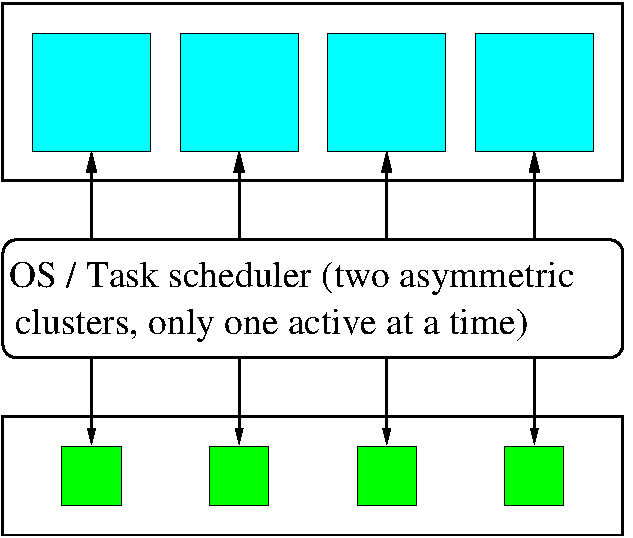
\includegraphics[width=0.4\textwidth]{Figures/Models/clustered.pdf}
   \caption{CSM}
  \end{subfigure}

	\medskip

  \begin{subfigure}{.75\textwidth}
   \centering
   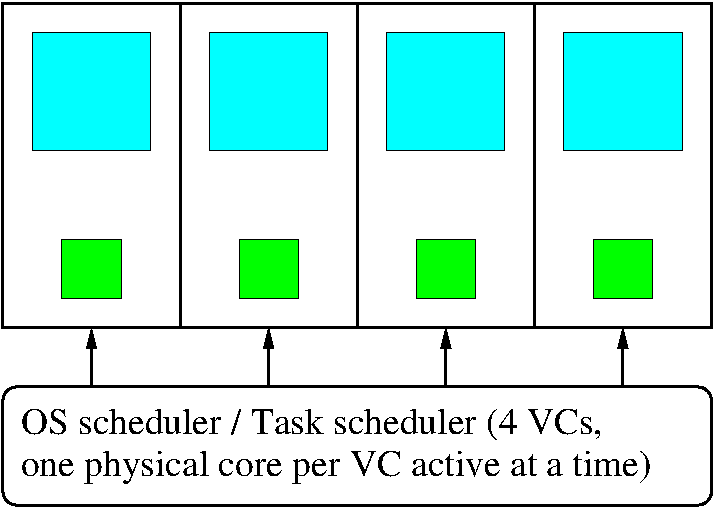
\includegraphics[width=0.45\textwidth]{Figures/Models/iks.pdf}
   \caption{CPUM}
  \end{subfigure}

	\medskip

  \begin{subfigure}{.75\textwidth}
   \centering
   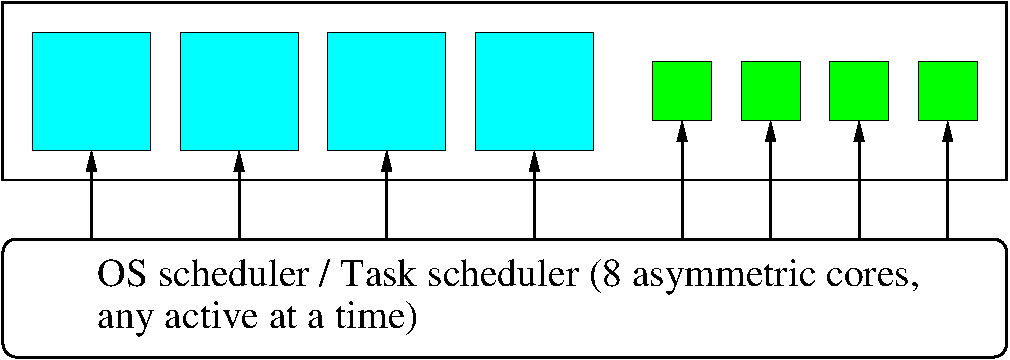
\includegraphics[width=0.6\textwidth]{Figures/Models/gts.pdf}
   \caption{GTS}
  \end{subfigure}
   \caption{Modos de operación de las arquitecturas big.LITTLE actuales.}
   \label{fig:modes}
\end{figure}

\comentario{Falta traducir figura}


La Figura~\ref{fig:modes} ofrece una visión esquemática de estos tres modelos de ejecución
sobre arquitecturas big.LITTLE modernas. GTS es la solución más flexible, ya que permite al planificador
del sistema operativo asignar hebras a cualquiera de los núcleos disponibles, es decir, todos
los núcleos disponibles se ofrecen al sistema operativo como candidatos a ejecutar el código
de cualquier hebra, independientemente de su naturaleza o características. Esta característica
permite migrar de forma muy sencilla aplicaciones multihebra ya existentes, incluyendo planificadores
de tareas en tiempo de ejecución, y explotar todos los recursos computacionales en este tipo de 
procesadores asimétricos, utilizando cualquier mecanismo estándar de creación y gestión de hebras
(por ejemplo, pthreads u OpenMP). Sin embargo, conseguir prestaciones óptimas no resulta tan
sencillo, especialmente en aplicaciones multihebra en las que el desequilibrio de carga introducido
por la asimetría de la arquitectura puede penalizar el rendimiento obtenido. Solucionar este problema
es uno de los objetivos de este trabajo.

De forma alternativa, CPUM propone una visión pseudosimétrica del procesador big.LITTLE; por ejemplo,
en el caso del SoC Exynos 5422, los 8 núcleos asimétricos son vistos de forma lógica como 4 grupos
de pares de procesadores, convirtiendo así la arquitectura en un sistema simétrico formado por
4 núcleos virtuales (VC), que son expuestos de esta manera al sistema operativo.

En la práctica, los planificadores de tareas en tiempo de ejecución pueden aproximar a nivel software
cualquiera de estos tres paradigmas. Un modelo trivial puede seguir las directivas de GTS para asignar
cualquier tarea lista para su ejecución a cualquiera de los núcleos disponibles en el sistema. Con esta
solución, el desequilibrio de carga podría resolverse desarrollando políticas de planificación a nivel
de tarea específicas (conscientes de la asimetría), para asignar tareas al recurso más apropiado en 
función de sus características. 

Sin embargo, este trabajo propone un enfoque alternativo, en el que el SoC asimétrico es visto de forma
lógica como un conjunto {\em simétrico} de núcleos virtuales, cada uno de ellos compuesto internamente
por distintos tipos de núcleo, pero considerado, de cara al planificador, como un sistema simétrico. Esto
facilita el desarrollo de políticas de planificación, como se verá más adelante, y permite incluso
reutilizar planificadores ya existentes sobre este tipo de arquitecturas.



%-- Configuraciones para emacs --
%%% Local Variables:
%%% mode: latex
%%% TeX-master: "./principal.tex"
%%% End:

\cleardoublepage

% \newpage
% \thispagestyle{empty}
% \mbox{}

\chapter{Modelos de programación basados en paralelismo a nivel de tareas}
\label{ch:chapter3}

\section{Descripción general y estado del arte}

\section{OmpSs}

\subsection{Modelo de programación}

\subsection{Planificador de tareas}

\subsection{Ejemplo. Factorización de Cholesky}


\section{Adaptación de OmpSs a arquitecturas asimétricas (botlev)}
%%
\comentario{Título: No se si adaptación, o ampliación, o incorporación, o uso de
  OmpSs sobre asim, o ...} %%
Con el reciente auge de las arquitecturas asimétricas en el mundo HPC, el
equipo de desarrollo de OmpSs ha introducido un nuevo planificador
denominado \emph{Bottom level-aware scheduler} (Botlev)~\cite{botlev}
específico para este nuevo tipo de arquitecturas. Botlev recoge las ideas
de los planificadores tradicionales basados en arquitecturas heterogéneas,
distinguiendo únicamente dos tipos de nodos de cómputo (un nodo rápido
formado por los cores de tipo big, y un nodo de cómputo lento formado por
los cores de tipo LITTLE) y eliminando el
cálculo de los costes asociados a la transferencia de datos. \\
La principal idea que se encuentra detrás de Botlev es la de detectar en
tiempo de ejecución qué tareas pertenecen al camino crítico y cuáles no, y
obligar a que los cores rápidos sean los encargados de ejecutar las tareas
del camino crítico. Además, en caso de existir alguna tarea perteneciente
al camino crítico lista para ser ejecutada, esta tendrá preferencia sobre
el resto de tareas que también estén listas para ejecución.\\
El objetivo de garantizar que las tareas del camino crítico se ejecutan en
los cores rápidos cuanto antes es asegurarse que al ejecutar las tareas
críticas, estas liberarán dependencias con nuevas tareas que pasarán a
estar listas para ejecución, y así intentar conseguir que nunca haya cores
ociosos, lo cual disminuiría el rendimiento global de la aplicación. La
principal diferencia entre botlev y los planificadores tradicionales para
sistemas heterogéneos es que botlev toma las decisiones en tiempo dinámico
sin necesidad de conocer de antemano información sobre las tareas, o al
forma del árbol de dependencias.

Para determinar si una tarea pertenece al camino crítico o no en tiempo de
ejecución, botlev asigna una prioridad a cada tarea en el momento de la
inserción en el grafo de dependencias. Una vez que la tarea está lista para
ser ejecutada (es decir, cuando todas las tareas que tenían relación con la
tarea mediante el grafo de dependencias han finalizado su ejecución), se
realiza la decisión de qué core va a ejecutar la tarea en función de la
prioridad
asignada.\\
La prioridad de una tarea viene dada por un número entero positivo, el cuál
representa la longitud del camino más largo desde la tarea actual hasta una
tarea hoja del grafo de dependencias. Cuando una tarea es introducida en el
grafo de dependencias, se le asigna una prioridad 0 ya que la longitud del
camino más largo desde la tarea a un nodo hoja (ella misma) es 0. Además,
cuando una tarea se inserta en el TDG, se actualizan las prioridades de
todas las tareas predecesoras, ya que estas pueden haber cambiado. Por cada
tarea predecesora, se intenta aumentar la prioridad en 1 unidad (el camino
es un nodo más largo), siempre que no tuviera una prioridad mayor antes
(este es el caso de que la tarea pertenezca a un camino más largo en el que
la nueva tarea no esté involucrada). El proceso de actualización finaliza
cuando se actualiza la tarea raíz del árbol, o cuando se alcanza una tarea
que pertenece a otro camino más largo que el actual. En la
figura~\ref{s3:fig:botlev_tdg} se puede ver el camino crítico detectado
para una factorización de Cholesky sobre una matriz dividida en $8\times8$
bloques. Hay que destacar que esta forma de calcular el camino crítico
detecta las tareas que pertenecen al camino más largo, pero eso no implica
que sean aquellas que más van a retrasar la ejecución en caso de que no se
ejecuten de manera prioritaria. Para calcular esto, sería necesario conocer
de antemano las necesidades de cada tarea, o ir almacenando resultados
parciales de ejecución de manera dinámica para tomar decisiones en el
futuro.
%%
\comentario{La figura de las colas no se ve muy bien.} %%
\begin{figure}
  \centering
  
  \begin{subfigure}{.45\textwidth}
    \centering
    \setlength{\fboxsep}{5pt}
    \fbox{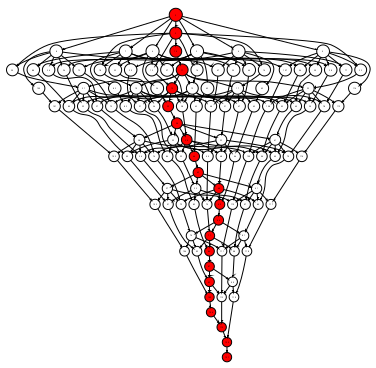
\includegraphics[width=.8\linewidth]{Figures/botlev-tdg.png}}
    \caption{Camino crítico en botlev para una factorización de Cholesky de
      $8\times8$ bloques.}
    \label{s3:fig:botlev_tdg}
  \end{subfigure}
  % Si se deja una línea en blanco, las coloca en vertical
  \begin{subfigure}{.45\textwidth}
    \centering
    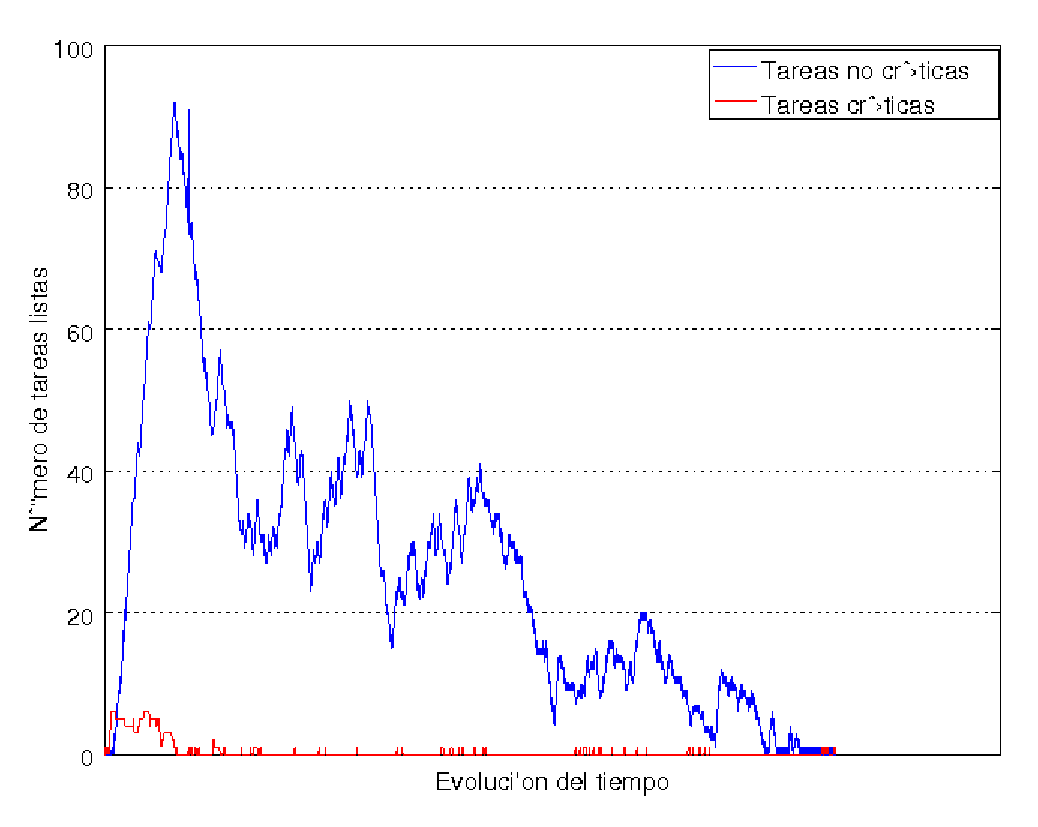
\includegraphics[width=1\linewidth]{Figures/botlev-colas.eps}
    \caption{Evolución del tamaño de las colas de tareas
      listas.\todo{agrandar texto}}
    \label{s3:fig:botlev_colas}
  \end{subfigure}  
  
  \caption{Cálculo de tareas críticas en Botlev y asignación a cores.}
  \label{s3:fig:botlev}
\end{figure}

Una tarea puede ser ejecutada cuando todas sus tareas predecesoras han
finalizado la ejecución. Cuando esto ocurre, Botlev inserta la tarea en una
cola de tareas pendientes para ir ejecutándolas en función de la prioridad
asignada, o en orden de insercción en caso de empate. Estas tareas son
asignadas a los diferentes cores según vayan finalizando la ejecución de
las tareas previas. Según la prioridad de la tarea, Botlev distingue dos
tipos de colas en las que insertar una tarea: la cola con las tareas
pertenecientes al camino crítico, y la cola con el resto de tareas. Una
tarea se considera que pertenece al camino crítico si posee una prioridad
mayor a cualquiera de las prioridades de las tareas anteriores, o si es
hija directa de una tarea que se ha considerado crítica y tiene una
prioridad de una unidad menor (es decir, es el siguiente nodo del camino
crítico). En la figura~\ref{s3:fig:botlev_colas} se puede ver la evolución
del tamaño de las colas para una factorización de Cholesky sobre una matriz
de $8\times8$ bloques. La línea azul muestra el número de tareas no
críticas listas para ser ejecutadas en función del momento de la ejecución
del problema, mientras que la línea roja muestra el
número de tareas críticas.

Cuando un core big finaliza la ejecución de una tarea, este ejecutará la
siguiente tarea de la cola de tareas críticas, mientras que un core LITTLE
ejecutará la primera tarea de la cola de tareas no críticas. De esta forma
se consigue asignar las tareas críticas a cores big, mientras que las
tareas no críticas serán ejecutadas por cores lentos. Para grafos de
dependencias muy anchos, como puede ser el asociado a una factorización de
Cholesky, el número de tareas críticas es mucho menor que el número de
tareas no críticas, dando lugar a que los cores rápidos estén la mayor
parte de tiempo ociosos. Para evitar esta situación, si un core big no
dispone de tareas críticas que ejecutar, ejecutará la siguiente tarea de la
lista de tareas no críticas. El robo de tareas en sentido contrario (es
decir, que los cores LITTLE ejecuten tareas críticas) es una parámetro
adicional que se puede seleccionar en tiempo de ejecución, pero que se
encuentra desactivado por defecto.





%-- Configuraciones para emacs --
%%% Local Variables:
%%% mode: latex
%%% TeX-master: "./principal.tex"
%%% End:

\cleardoublepage
% \newpage
% \thispagestyle{empty}
% \mbox{}

\chapter{Optimización del rendimiento de OmpSs sobre arquitecturas asimétricas}
\label{ch:chapter4}

%\section{Descripción de la estrategia de optimización}
%
%\section{BLIS}
%
%\subsection{Adaptación de BLIS a arquitecturas asimétricas}
%
%\section{Combinación de BLIS asimétrico con OmpSs}
%
\section{Planteamiento y objetivos generales}

(Plantear objetivos e idea general. En el capítulo 5, copiaremos esta estructura, con la
misma sección inicial de motivación/objetivos).

In this section, we initially perform an evaluation 
of the task-parallel Cholesky routine in Listings~\ref{lst:chol}--\ref{lst:chol_tasks},
executed on top of the conventional (i.e., default) scheduler in 
OmpSs linked to a sequential instance of BLIS,  on the target Exynos 5422 SoC.  The outcome from this study 
motivates the development effort and experiments presented in the remainder of the paper.

\subsection{Evaluación de runtimes convencionales en AMPs}

La Figura~\ref{fig:ompss_blis_oversubscription} muestra el rendimiento, en términos de GFLOPS (miles de millones de
operaciones en coma flotante por segundo), mostrado por el runtime convencional de OmpSs para la factorización
de Cholesky, variando el número de \wts entre~1 y~8 sobre la plataforma asimétrica \odroid; en el 
experimento, se delega la asignación de \wts a núcleos al planificador del sistema operativo. En otras palabras,
se está utilizando una versión no consciente de la asimetría del planificador de tareas en OmpSs.
Para este experimento, se ha evaluado un rango lo suficientemente amplio de tamaños de bloque 
({\tt b} en el código de la Figura~\ref{lst:chol}), aunque por simplicidad se reporta únicamente los
resultados obtenidos para el valor de {\tt b} que optimiza el ratio de GFLOPS para cada dimensión
del problema\footnote{En este capítulo, todos los experimentos se han realizado utilizando doble precisión.}.

\begin{figure}
\centering
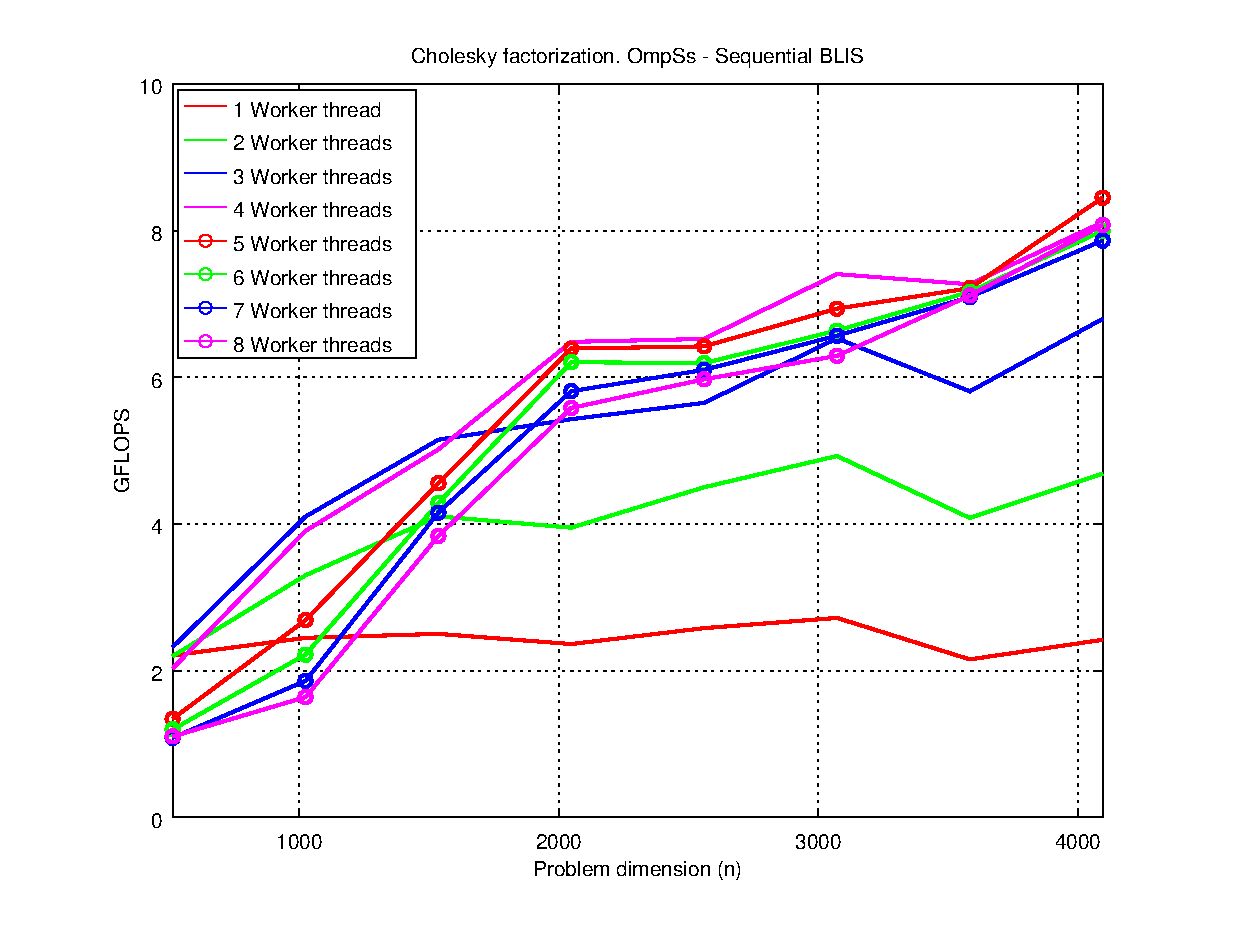
\includegraphics[width=0.70\textwidth]{Plots/Orig_runtime/plot_1to8_th}
\caption{Rendimiento de la factorización de Cholesky utilizando el runtime OmpSs convencional y una implementación secuencial
	de BLIS sobre el SoC Exynos 5422.}
\label{fig:ompss_blis_oversubscription}
\end{figure}

%All the experiments hereafter employed {\sc ieee} double precision. Furthermore,
%we  ensured that the cores operate at the highest possible frequency by setting the appropriate {\em cpufreq} governor.
%The conventional runtime of OmpSs corresponds to release 15.06 of the Nanos++ runtime task scheduler.
%For this experiment, it is lined with the ``sequential'' implementation of BLIS in release 0.1.5.
%(For the experiments with the multi-threaded/asymmetric version of BLIS in the later sections, 
%we will use specialized versions of the codes in~\cite{asymBLIS} for slow+fast VCs.)

Los resultados experimentales revelan un incremento en el rendimiento a medida que el número de \wts aumenta entre~1 y~4,
casos en los que el planificador del sistema operativo asigna su ejecución a los núcleos rápidos (Cortex-A15) disponibles.
Sin embargo, cuando el número de \wts excede la cantidad de núcleos rápidos, el sistema operativo se ve forzado a asignar
\wts a núcleos lentos (Cortex-A7), en cuyo caso el aumento en prestaciones desaparece, e incluso éstas disminuyen drásticamente 
a medida que el número de \wts aumenta. La principal causa de este decremento en las prestaciones es el desequilibrio de carga,
ya que tareas con granularidad uniforme, posiblemente pertenecientes al camino crítico, son asignadas a núcleos lentos.

Este experimento revela la principal motivación por la que es necesario un planificador de tareas consciente de la
arquitectura y adaptado a ella~\cite{OmpSsbigLITTLE}. Sin embargo, en el presente capítulo, se desarrollará un enfoque alternativo
a la hora de explotar la asimetría de la arquitectura subyacente: se utilizará un planificador de tareas convencional en combinación
con una biblioteca asimétrica para la ejecución de tareas, como se describe a continuación.

\section{Combinación de runtimes convencionales con bibliotecas asimétricas}

\subsection{Visión general de la propuesta}

La propuesta de operación introducida en el presente capítulo opera bajo el modelo GTS, pero está en cierto modo 
inspirada en el modelo CPUM (véase Sección~\ref{sec:models}). Más concretamente, el objetivo es que el planificador
de tareas considere la arquitectura \odroid (por ejemplo) como una arquitectura verdaderamente simétrica, formada por 
cuatro VCs (núcleos virtuales, o {\em Virtual Cores}), cada uno de ellos compuesto por un núcleo rápido y un núcleo
lento. Para ello, a diferencia del modelo CPUM, {\em ambos} núcleos físicos dentro de cada VC se mantendrán activos y 
colaborarán en la ejecución de una determinada tarea. Así, la propuesta explota dos niveles de concurrencia: el {\em paralelismo
a nivel de tareas} es extraído por el planificador para asignar tareas a cada uno de los cuatro VCs idénticos disponibles en
el sistema, e internamente, cada tarea/kernel divide su carga de forma correcta para exponer {\em paralelismo a nivel de datos}, 
distribuyendo la carga de trabajo entre los dos núcleos físicos asimétricos dentro del VC que está a cargo de la ejecución
de dicha tarea.

Esta solución requiere únicamente un planificador de tareas convencional (es decir, no consciente de la asimetría de la arquitectura, o lo
que es lo mismo, orientado a arquitecturas SMT), como por ejemplo el planificador de tareas convencional proporcionado por OmpSs, donde, 
en lugar de crear un \wt\ por núcleo físico del sistema, se sigue una filosofía similar a la propuesta por el modelo CPUM, creando 
{\em un único worker thread por VC}. Internamente, cuando una tarea es elegida para ser ejecutada por un \wt disponible, dicha tarea
se ejecutará, de forma ya no secuencial, sino paralela sobre cada uno de los núcleos que componen el VC, explotando, en este caso,
la asimetría interna de dicha abstracción. Por ejemplo, en el caso de \odroid, equipada con cuatro núcleos rápidos y cuatro lentos, 
la propuesta desarrollada desplegará únicamente cuatro \wts; para cualquier tarea básica o kernel de álgebra lineal a ejecutar, dicha
rutina explotará la asimetría internamente, siempre bajo la condición de que existe una implementación de la misma optimizada para
este tipo de paralelismo asimétrico.

Siguiendo esta idea, la arquitectura expuesta al planificador de tareas es completamente {\em simétrica}, y los kernels en BLIS
(o en cualquier otra biblioteca utilizada para la ejecución de las tareas) configuran una ``caja negra'' que abstrae del carácter
asimétrico al planificador.

En resumen, si en una configuración convencional el núcleo es el recurso mínimo de computación para el planificador de tareas,
y éstas son totalmente secuenciales, en la solución propuesta el VC es el recurso básico de computación de cara al planificador,
mientras que la implementación de las tareas pasa a ser no sólo paralela, sino adaptada para la correcta explotación del paralelismo
existente dentro de cada VC.

\subsection{Comparación y ventajas frente a otras alternativas}


%Provided an underlying asymmetry-aware library is available to the developer, it is possible to combine this 
%with an existing conventional runtime task scheduler in order to exploit the underlying architecture. 
%In the enhanced version of OmpSs in~\cite{OmpSsbigLITTLE}, tasks were actually invocations to a {\em sequential} 
%library implementation, and asymmetry was exploited via sophisticated scheduling policies specially designed for asymmetric architectures. 
%Following our new approach, asymmetry is exploited at the library level, not at the runtime level. 
%To accommodate this, tasks are cast in terms of 
%invocations to a multi-threaded asymmetry-aware library (in our case, BLIS). 

La solución desarrollada reúne un conjunto de ventajas de cara al desarrollador:

\begin{itemize}
\item El planificador de tareas no es consciente de la asimetría, por lo que cualquier versión convencional 
      del mismo podrá trabajar sobre este tipo de sistemas sin modificaciones específicas. 
\item Cualquier política de planificación (por ejemplo, {\em work stealing}, planificación consciente de la localidad de datos,
      implementación de caches por software, \ldots) ya desarrollada para arquitecturas simétricas, o cualquier futura mejora,
      tendrá también un impacto directo en el rendimiento sobre el sistema asimétrico.
\item Cualquier mejora en la implementación de las bibliotecas asimétricas subyacentes (por ejemplo, BLIS) tendrá un impacto directo
      sobre el AMP. Esta observación se aplica a arquitecturas con distinto número de núcleos lentos/rápidos dentro del VC, ratios
      en las frecuencias de funcionamiento, o incluso ante la introducción de más niveles de asimetría (esto es, núcleos con rendimiento
      intermedio).
\end{itemize}

Obviamente, existe una dificultad adicional intrínseca a la solución propuesta, y que se convierte en un requisito fundamental de cara
a su viabilidad: debe existir, necesariamente, una versión consciente de la asimetría para cada tarea a ejecutar (por ejemplo, una implementación
completa de las rutinas BLAS). En el ámbito del álgebra lineal densa, este requisito se cumple a través de la versión asimétrica de BLIS, aunque
en otros ámbitos, el desarrollo específico de este tipo de implementaciones es todavía escaso.

\subsection{Requisitos a nivel de tarea en el ámbito del álgebra lineal}

\comentario{Hay que reescribir esta sección}.

Por último, cabe destacar que son necesarios ciertos requisitos adicionales en la implementación multihebra de BLIS
que opera sobre el modelo propuesto. Considérese el kernel \gemm y la descripción de alto nivel proporcionada en la Figura~\ref{lst:gemm}. 
Como se ha descrito anteriormente, resulta necesario distribuir el espacio de iteraciones de alguno de los bucles entre los dos tipos de núcleos
que conforman un VC; siguiendo las directivas de paralelización descritas en~\cite{BLIS3}, se distinguen a continuación dos escenarios de reparto posibles:

\begin{itemize}
	\item En arquitecturas donde cada VC está compuesto por igual número de núcleos de cada tipo (por ejemplo, \odroid) \ldots

	\item En arquitecturas donde cada VC está compuesto por distinto número de núcleos de cada tipo (por ejemplo, \juno) \ldots

\end{itemize}

For our objective, we still have to distribute the iteration space between the Cortex-A15 and the Cortex-A7 but, since there is only one resource of each type per VC,
there is no need to partition the loops internal to the macro-kernel. 
Furthermore, we note that the optimal strides for Loop~1 are in practice quite
large ({\tt nc} is in the order of a few thousands for ARM big.LITTLE cores), while the optimal values for Loop~3 are much more reduced
({\tt mc} is 32 for the Cortex-A7 and 156 for the Cortex-A15). Therefore, we target Loop~3 in our data-parallel implementation of BLIS for
VCs, which we can expect to easily yield a proper workload balancing.

%That is, both the number of cores to use, and the distribution of those cores between the fast and slow processing units are transparent and 
%fully configurable by the user. 

\section{Resultados experimentales}

\subsection{Estudio experimental del tamaño de bloque óptimo}

En tiempo de ejecución, OmpSs descompone la rutina para la implementación de la factorización de Cholesky en una colección de tareas
que operan en submatrices (bloques) con una granularidad que viene definida por el tamaño de bloque {\tt b}, véase el código en la 
Figura~\ref{lst:chol}. Estas tareas típicamente se reducen a invocaciones a kernels elementales a nivel de BLAS (en nuestro caso,
BLIS) o LAPACK, véase el código proporcionado en la Figura~\ref{lst:chol_tasks}.  

\newcommand{\bopt}{b^{\mbox{\rm \scriptsize opt}}\xspace}

El primer paso en nuestra evaluación radica en proporcionar una estimación realista de la ganancia de rendimiento
potencial proporcionada por la solución propuesta (en caso de haberla). Un factor crítico desde este punto de vista es
el rango de tamaños de bloque que resultan óptimos para el runtime convencional de OmpSs ante una determinada operación
(en adelante $\bopt$). En particular, la eficiencia de la solución propuesta vendrá determinada por el rendimiento obtenido
por las implementaciones BLIS de cada una de las tareas que componen la operación, comparada con su implementación secuencial
equivalente para dimensiones del problema {\tt n} en el orden de dimensión $bopt$.

La Tabla~\ref{tab:optimal_bs_sym} muestra los tamaños de bloque óptimos $\bopt$ para la factorización de Cholesky y tamaños
de problema crecientes, utilizando el planificador OmpSs convencional enlazado con una versión secuencial de BLIS y un número
creciente de \wts entre~1 y~4. Obsérvese como, excepto para los menores tamaños de problema, los tamaños de bloque óptimos están
en el rango entre 192 y 448. Estos tamaños de bloque resultan óptimos al ofrecer un equilibrio entre el paralelismo a nivel de tareas
potencial y la eficiencia interna de las ejecuciones secuenciales de cada tarea individual.

\newcommand{\ra}[1]{\renewcommand{\arraystretch}{#1}}
\newcommand{\ca}[1]{\renewcommand{\tabcolsep}{#1}}

\ra{1.2}
\ca{2pt}

\begin{table}
	\centering
	\caption{Tamaños de bloque óptimos para la factorización de Cholesky utilizando el planificador convencional
	         de OmpSs y una implementación secuencial de BLIS sobre \odroid.}
	\label{tab:optimal_bs_sym}
{\scriptsize
\begin{tabular}{crrrrrrrrrrrrrrrr} 
\toprule
  & \phantom{a} & \multicolumn{14}{c}{Tamaño del problema ({\tt n})} \\ 
\cmidrule{3-17} 
  & \phantom{a} &     512 & 1,024 & 1,536 & 2,048 & 2,560 & 3,072 & 3,584 & 4,096 & 4,608 & 5,120 & 5,632 & 6,144 & 6,656 & 7,168 & 7,680 \\ \hline

{\sc 1 wt} & \phantom{a} &     192 & 384  & 320  & 448  & 448  & 448  & 384  & 320 & 320 & 448 & 448 & 448 & 448 & 384 & 448 \\ \hline
{\sc 2 wt} & \phantom{a} &     192 & 192  & 320  & 192  & 448  & 448  & 384  & 320 & 320 & 448 & 448 & 448 & 448 & 384 & 448 \\ \hline
{\sc 3 wt} & \phantom{a} &     128 & 192  & 320  & 192  & 384  & 448  & 320  & 320 & 320 & 448 & 448 & 448 & 448 & 384 & 448 \\ \hline
{\sc 4 wt} & \phantom{a} &     128 & 128  & 192  & 192  & 192  & 320  & 320  & 320 & 320 & 448 & 320 & 448 & 448 & 384 & 448 \\ \bottomrule
\end{tabular}
}
\end{table}

La principal conclusión extraída tras el análisis de los resultados es la siguiente: para elevar el rendimiento de un planificador
de tareas combinado con una versión asimétrica de BLIS, cada uno de los kernels que componen la operación implementados en dicha
versión asimétrica debe exhibir mayor rendimiento que las respectivas implementaciones secuenciales, para dimensiones de matrices 
que estén en el orden de los tamaños de bloque mostrados en la Tabla~\ref{tab:optimal_bs_sym}.  

La Figura~\ref{fig:cross_blis} muestra el rendimiento alcanzado para las tres rutinas básicas BLAS que componen la factorización
de Cholesky (\gemm, \syrk y \trsm) para el rango de dimensiones de interés sobre la plataforma \odroid.  
El experimento compara la versión secuencial de BLIS sobre un único núcleo Cortex-A15 con la versión asimétrica de BLIS
que combina un Cortex-A15 y un Cortex-A7. Es decir, compara la ejecución de las tareas que componen la factorización sobre un
único núcleo físico (rápido) y sobre un VC (combinando un núcleo rápido y otro lento).

En general, las tres rutinas BLAS muestran una tendencia similar: los kernels de la versión secuencial de BLIS
consiguen mejor rendimiento que sus respectivas implementaciones asimétricas para tamaños de problema pequeños (hasta
aproximadamente {\tt m}, {\tt n}, {\tt k } = 128); sin embargo, 
a partir de dicha dimensión, el uso de un núcleo lento comienza a hacer que el rendimiento mejore. 
El aspecto más importante radica en el hecho de que el punto de corte entre ambas curvas está en el rango (e incluso 
es típicamente menor) de $\bopt$, véase Tabla~\ref{tab:optimal_bs_sym}. 
Esto implica que la versión asimétrica de BLIS puede, potencialmente, mejorar el rendimiento general de la factorización, 
incluso usando un planificador de tareas convencional.
Además, la mejora en rendimiento aumenta con el tamaño de problema, estabilizándose para dimensiones alrededor de 
{\tt m}, {\tt n}, {\tt k } $\approx~400$. Dado que este valor está en el rango del tamaño de bloque óptimo para
la factorización de Cholesky, sobre esta arquitectura es esperable una mejora en el orden de 0.3--0.5 GFLOPS por núcleo lento
añadido.
%mimicking the behavior of the underlying BLIS.

\begin{figure}[t]
\centering
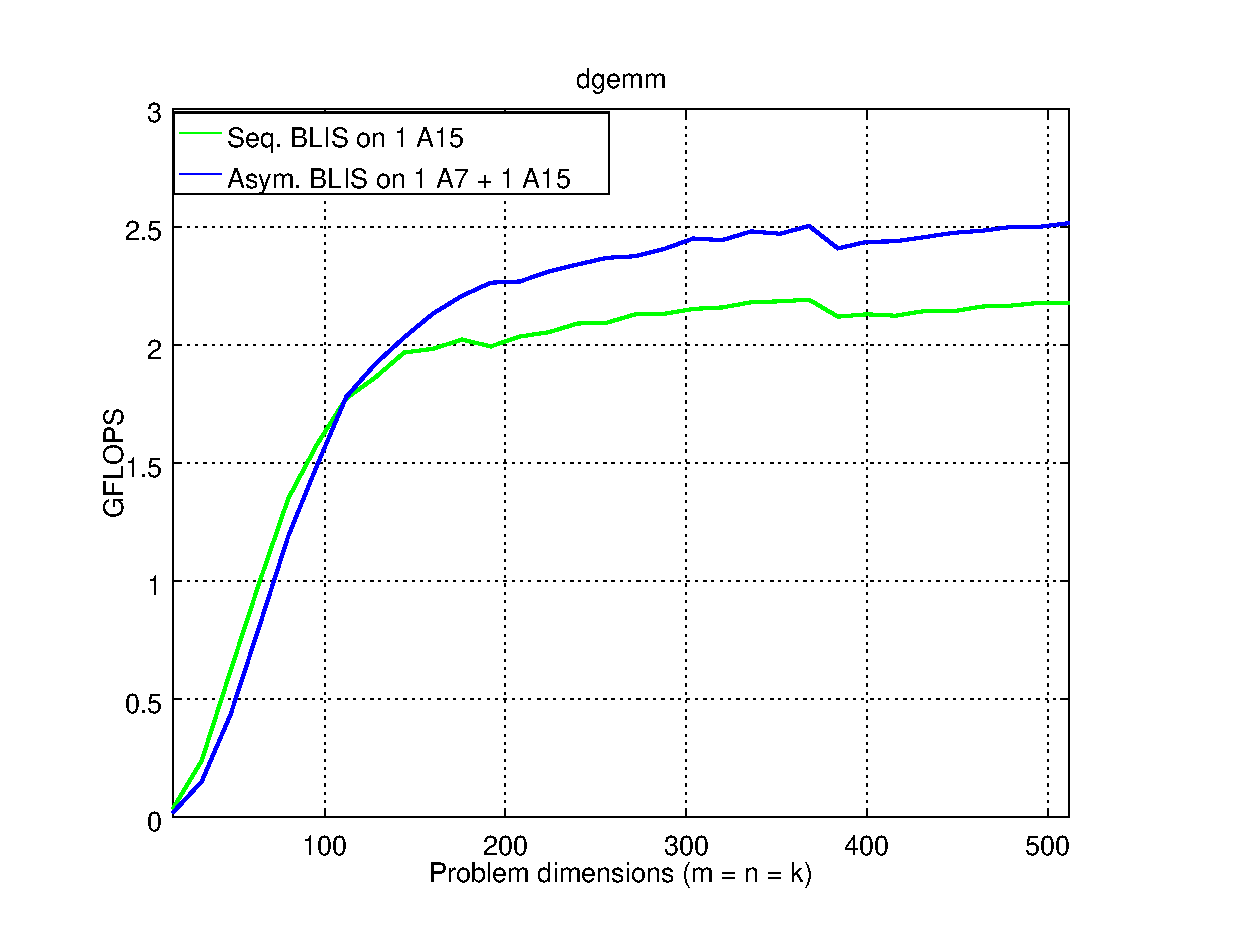
\includegraphics[width=0.49\textwidth]{Plots/BLIS_small/blis_dgemm_sym_asym}
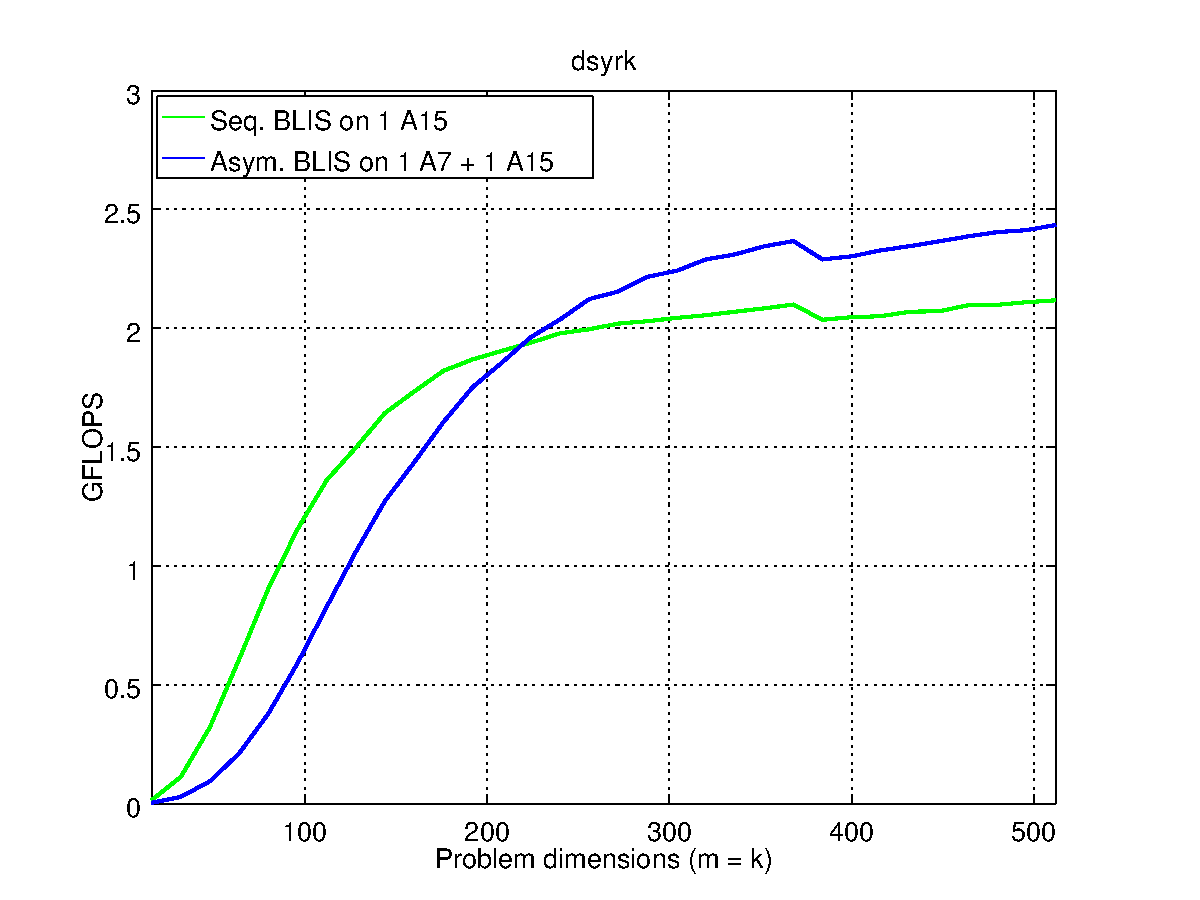
\includegraphics[width=0.49\textwidth]{Plots/BLIS_small/blis_dsyrk_sym_asym}
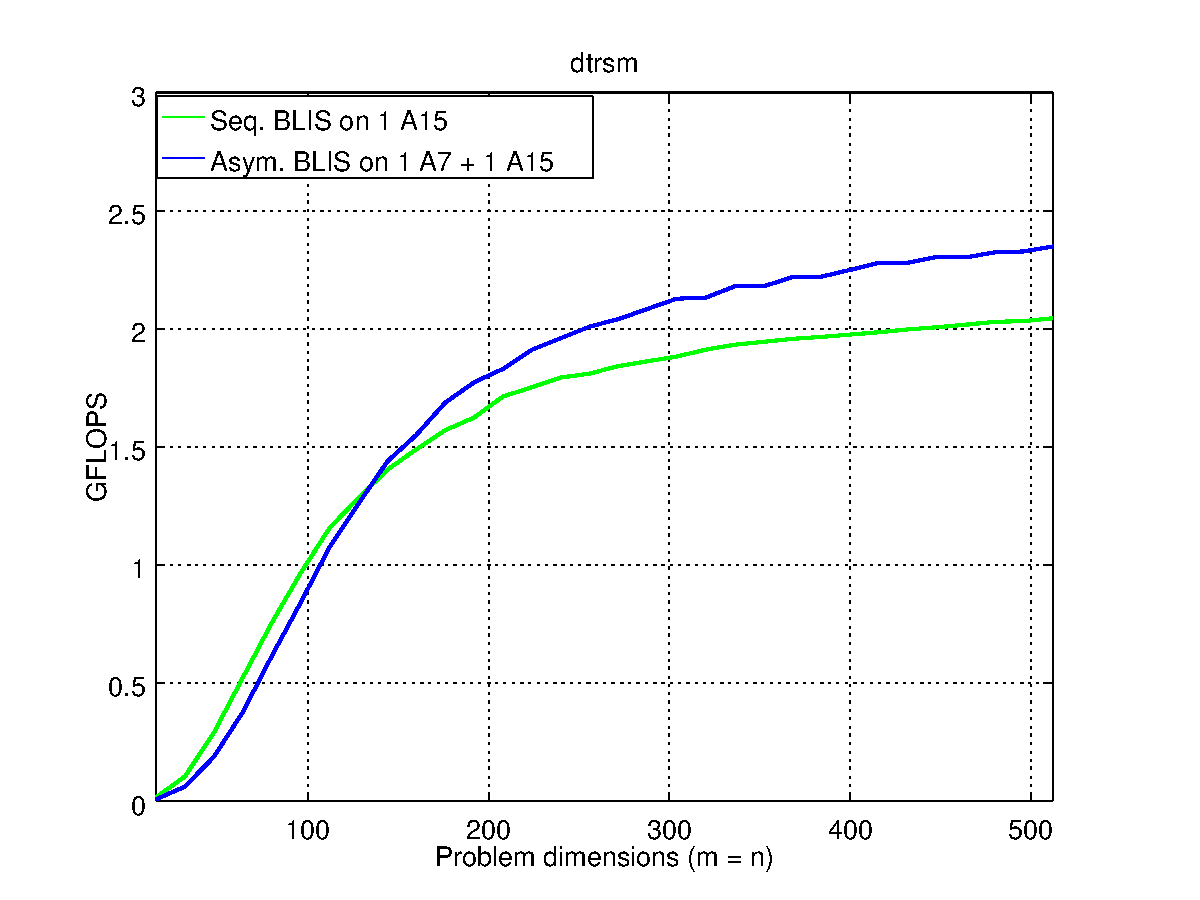
\includegraphics[width=0.49\textwidth]{Plots/BLIS_small/blis_dtrsm_sym_asym}
\caption{Rendimiento de los kernels BLAS-3 en las implementaciones secuencial y asimétrica de BLIS, utilizando, respectivamente
         un núcleo Cortex-A15 y un núcleo Cortex-A15 más un núcleo Cortex-A7 sobre \odroid.}
\label{fig:cross_blis}
\end{figure}


\subsection{Integración de BLIS asimétrico con un planificador de tareas convencional}

Con el fin de analizar los beneficios reales de la solución propuesta en términos de rendimiento, comparamos a continuación
el rendimiento del planificador OmpSs enlazado con {\em (a)} una versión secuencial de BLIS, y {\em (b)} con la versión asimétrica de BLIS. 
En todos los experimentos, los kernels BLIS en la primera configuración utilizaran exclusivamente un núcleo Cortex-A15, mientras
que en el segundo caso se utilizara un núcleo Cortex-A15 más un núcleo Cortex-A7 para la ejecución de las tareas.
%
La Figura~\ref{fig:ompss_blis} muestra los resultados obtenidos para ambas configuraciones, utilizando un número creciente
de \wts, entre~1 y~4. Por simplicidad, únicamente se reportan los resultados obtenidos considerando el tamaño de bloque óptimo
para cada tamaño de problema. En todos los casos, la solución basada en la utilización de una biblioteca asimétrica mejora
el rendimiento de la implementación secuencial para matrices relativamente grandes (típicamente con dimensiones {\tt n}~$>$~2,048)
mientras que, para tamaños de problema menores, el ratio de GFLOPS obtenido en ambos casos es similar. 
La razón de este comportamiento viene marcada por el tamaño de bloque óptimo reportado en la Tabla~\ref{tab:optimal_bs_sym}
y el rendimiento de BLIS mostrado en la Figura~\ref{fig:cross_blis}: para dicho rango de dimensiones de problema,
el tamaño óptimo de bloque es significativamente menor, y ambas implementaciones BLIS obtienen resultados de rendimiento similares.

\begin{figure}%[t]
\centering
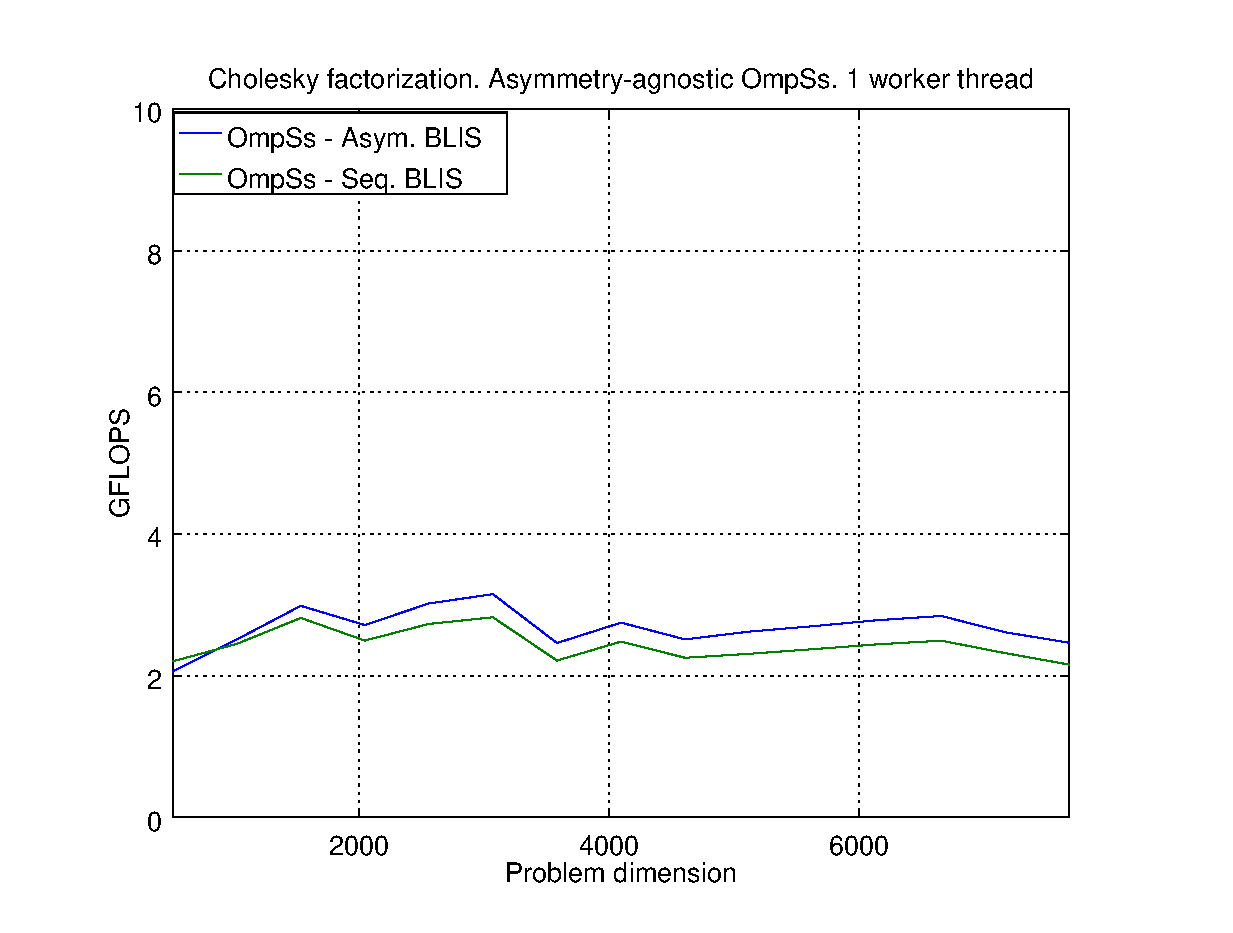
\includegraphics[width=0.49\textwidth]{Plots/Orig_runtime/plot_1_th}
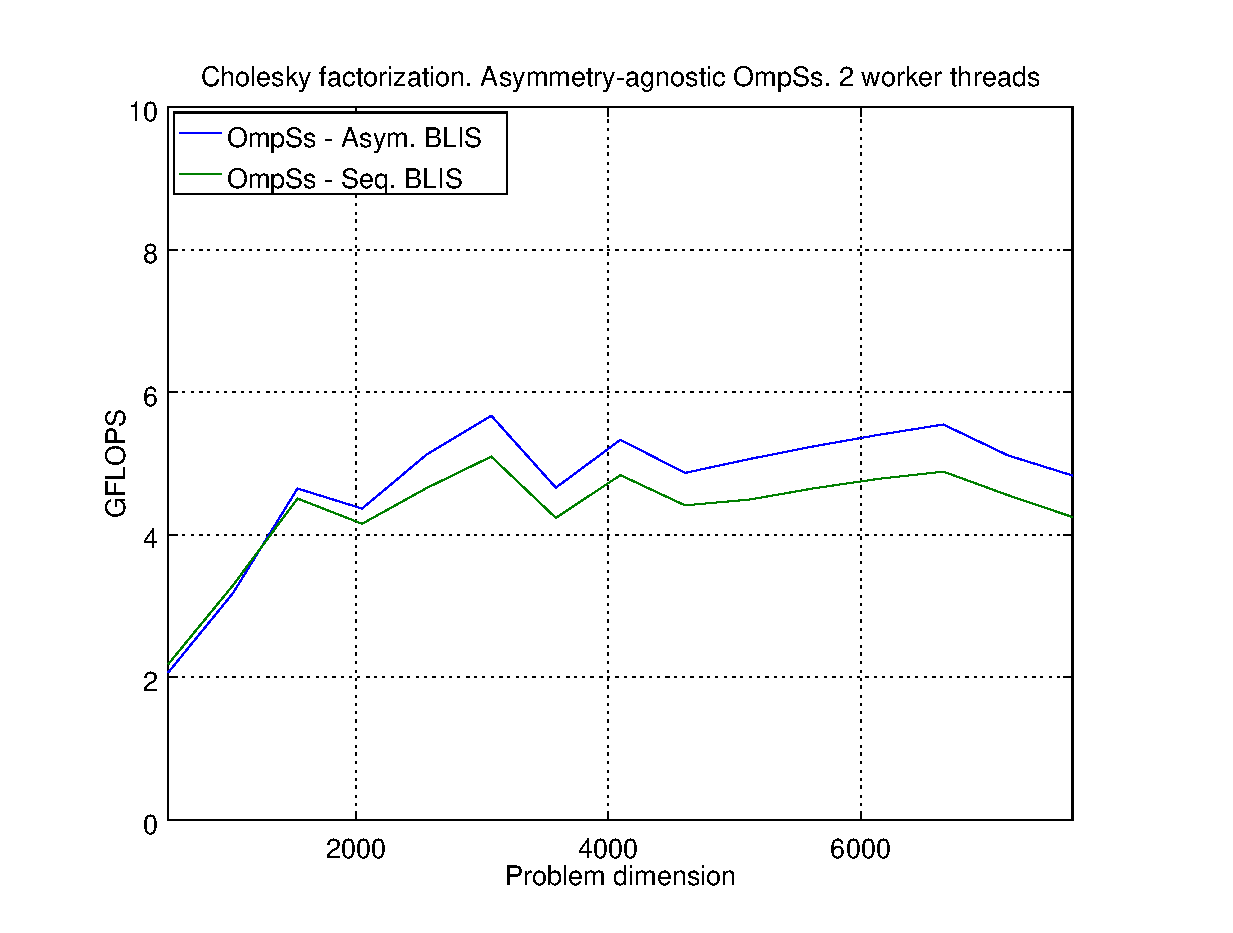
\includegraphics[width=0.49\textwidth]{Plots/Orig_runtime/plot_2_th}
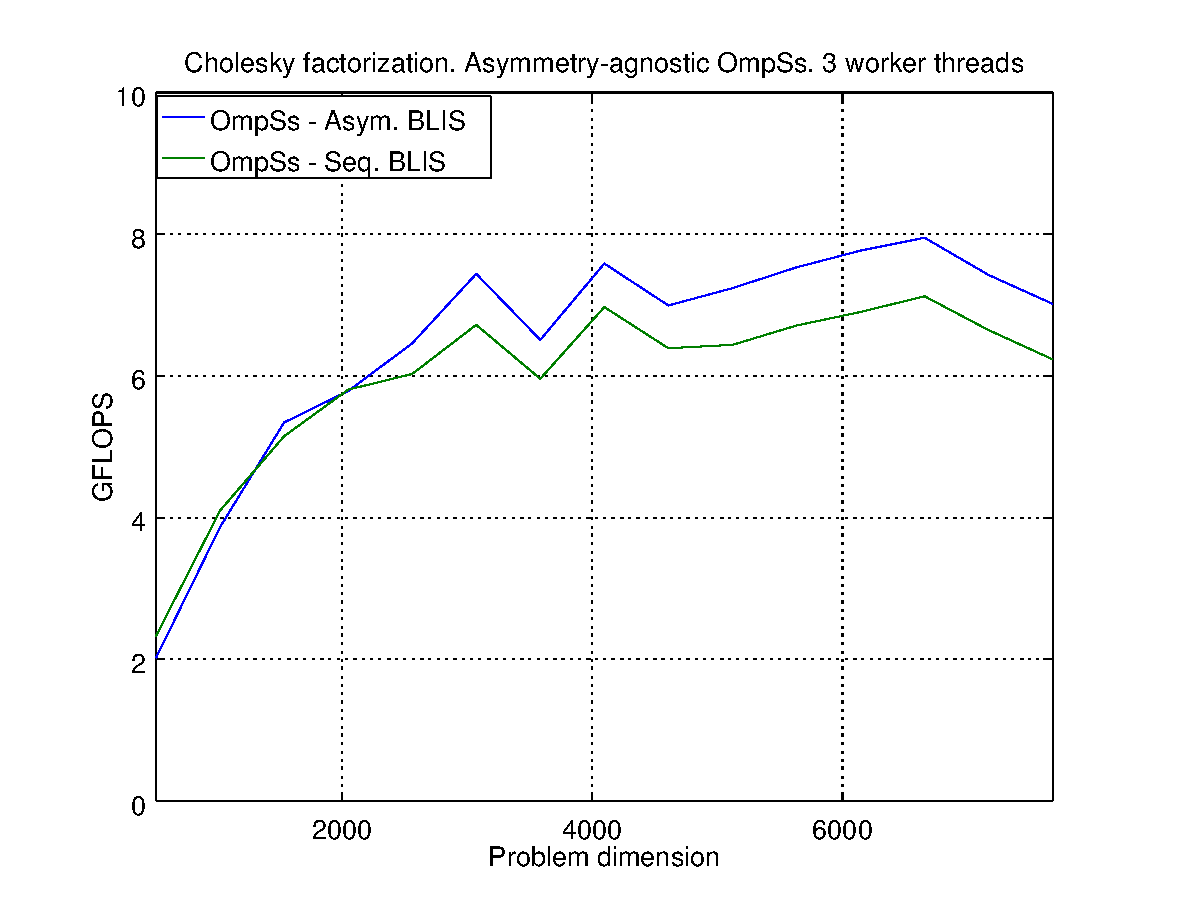
\includegraphics[width=0.49\textwidth]{Plots/Orig_runtime/plot_3_th}
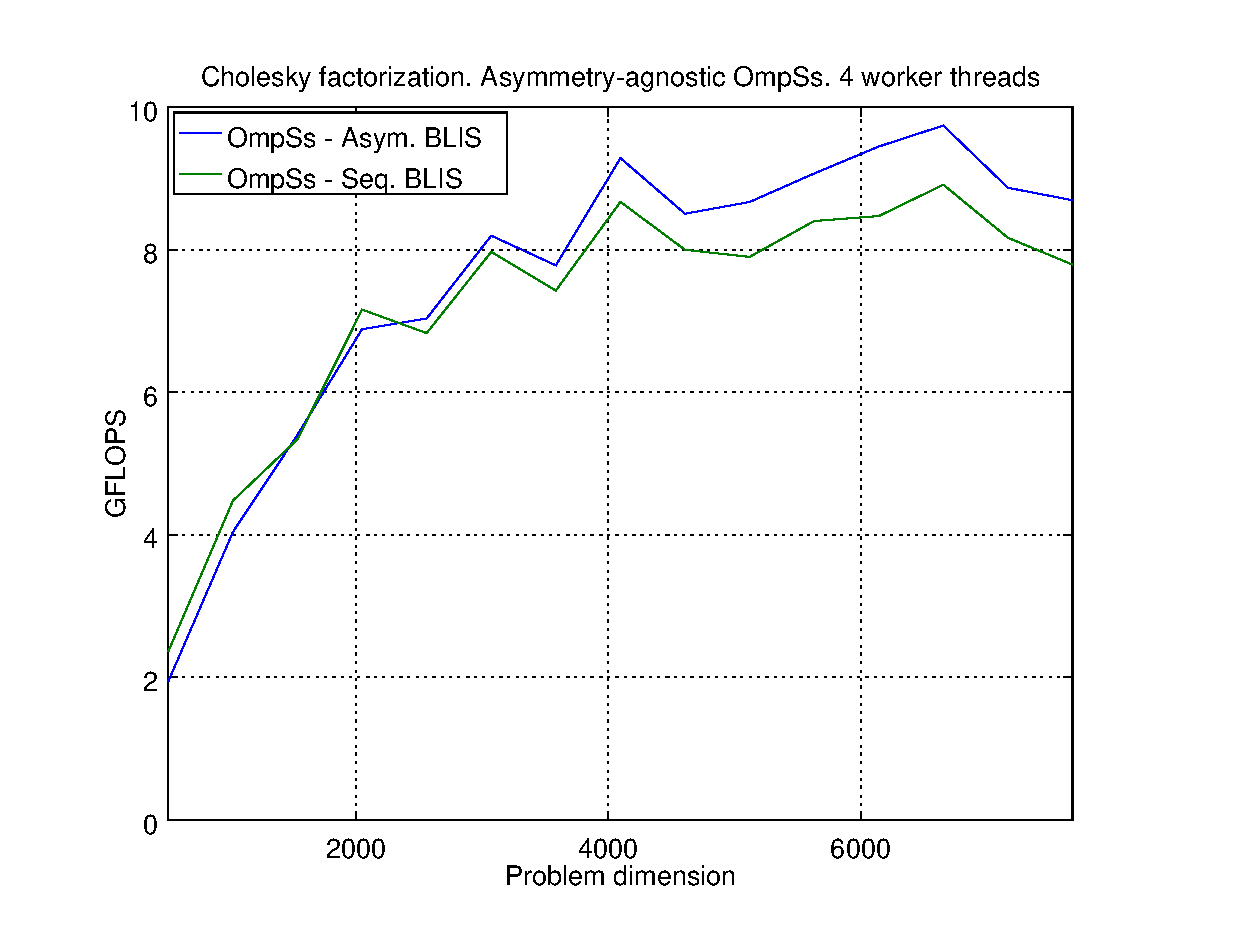
\includegraphics[width=0.49\textwidth]{Plots/Orig_runtime/plot_4_th}
\caption{Rendimiento de la factorización de Cholesky utilizando el planificador convencional de OmpSs, enlazado
         con la versión secuencial y asimétrica de BLIS.}
\label{fig:ompss_blis}
\end{figure}


%Table~\ref{tab:optimal_bs_sym}\ldots
%
%\begin{table}
	%\centering
	%\caption{Optimal block sizes for the Cholesky factorization using asymmetric BLIS.}
	%\label{tab:optimal_bs_asym}
	%\begin{tabular}{|c||c|c|c|c|c|c|c|c|c|c|c|c|c|c|c|}
		%\hline
		 %Th. &    512 & 1024 & 1536 & 2048 & 2560 & 3072 & 3584 & 4096 & 4608 & 5120 & 5632 & 6144 & 6656 & 7168 & 7680 \\ \hline \hline
		 %1   &    192 & 384 & 320 & 448 & 448 & 448 & 384 & 320 & 448 & 448 & 448 & 448 & 448 & 384 & 448 \\ \hline
		 %2   &    192 & 192 & 320 & 320 & 448 & 448 & 384 & 320 & 320 & 448 & 448 & 448 & 448 & 384 & 448 \\ \hline
		 %3   &    192 & 192 & 320 & 192 & 384 & 448 & 384 & 320 & 320 & 448 & 448 & 448 & 448 & 384 & 448 \\ \hline
		 %4   &    192 & 192 & 320 & 192 & 384 & 320 & 320 & 320 & 320 & 448 & 448 & 448 & 448 & 384 & 448 \\ \hline
	%\end{tabular}
%
%\end{table}

La diferencia cuantitativa en términos de rendimiento entre ambos enfoques se muestra
en las Tablas~\ref{tab:improvement_absolute} y~\ref{tab:improvement_percore}. 
La primera tabla muestra la diferencia absoluta en rendimiento, mientras que la segunda 
muestra la diferencia en rendimiento por cada núcleo lento (Cortex-A7) introducido en
el experimento. Consideremos, por ejemplo, el tamaño de problema {\tt n}~=~6,144. 
En este caso, el rendimiento mejora en 0.975 GFLOPS cuando se añaden los 4~núcleos lentos para 
dar soporte a los 4~núcleos Cortex-A15. Este hecho se traduce en una ganancia de rendimiento de
0.243 GFLOPS por core lento, ligeramente por debajo de la mejora que podría esperarse a partir de
los resultados experimentales observados en la anterior sección. Nótese, sin embargo, cómo el 
rendimiento por Cortex-A7 añadido se reduce desde 0.340~GFLOPS al añadir únicamente un núcleo,
hasta 0.243~GFLOPS, al utilizar los cuatro núcleos lentos.

\newcommand{\fg}[1]{\textcolor{ForestGreen}{#1}} % Verde
\newcommand{\br}[1]{\textcolor{BrickRed}{#1}} % Rojo

\begin{table}
	\centering
\caption{Mejora de rendimiento absoluta (en GFLOPS) para la factorización de Cholesky utilizando
         el planificador OmpSs convencional enlazado con una versión asimétrica de BLIS, con respecto
	 al mismo planificador enlazado con la versión secuencial de BLIS sobre \odroid.}
	 \label{tab:improvement_absolute}

%\begin{tabular}{|c||c|c|c|c|c|c|c|c|c|c|c|c|c|} 
   	%\hline
	%Th. &        512    & 1024       & 2048     & 2560     & 3072      & 4096     & 4608     & 5120    & 5632    & 6144     & 6656     & 7168     & 7680 \\ \hline \hline
	%1   &     -0.143    & 0.061      & 0.218    & 0.289    & 0.326     & 0.267    & 0.259    & 0.313   & 0.324   & 0.340    & 0.348    & 0.294    & 0.300    \\ \hline
	%2   &     -0.116    & -0.109     & 0.213    & 0.469    & 0.573     & 0.495    & 0.454    & 0.568   & 0.588   & 0.617    & 0.660    & 0.558    & 0.582    \\ \hline
	%3   &     -0.308    & -0.233     & -0.020   & 0.432    & 0.720     & 0.614    & 0.603    & 0.800   & 0.820   & 0.866    & 0.825    & 0.777    & 0.78    \\ \hline
	%4   &     -0.421    & -0.440     & -0.274   & 0.204    & 0.227     & 0.614    & 0.506    & 0.769   & 0.666   & 0.975    & 0.829    & 0.701    & 0.902    \\ \hline
%\end{tabular}
%%\end{table}

\ra{1.2}
\ca{2pt}

{\scriptsize
\begin{tabular}{crrrrrrrrrrrrr} 
   	\toprule
                 & \phantom{a} & \multicolumn{12}{c}{Dimensión del problema ({\tt n})} \\ 
\cmidrule{3-14} 
     & \phantom{a} &       512      & 1,024        & 2,048          & 2,560        & 3,072        & 4,096        & 4,608        & 5,120        & 5,632        & 6,144        & 6,656         & 7,680 \\ \hline 
{\sc 1 wt} & \phantom{a} &    \br{-0.143} & \fg{0.061}  & \fg{0.218}    & \fg{0.289}  & \fg{0.326}  & \fg{0.267}  & \fg{0.259}  & \fg{0.313}  & \fg{0.324}  & \fg{0.340}  & \fg{0.348}   & \fg{0.300} \\ \cline{3-14}
{\sc 2 wt} & \phantom{a} &    \br{-0.116} & \br{-0.109} & \fg{0.213}    & \fg{0.469}  & \fg{0.573}  & \fg{0.495}  & \fg{0.454}  & \fg{0.568}  & \fg{0.588}  & \fg{0.617}  & \fg{0.660}   & \fg{0.582} \\ \cline{3-14}
{\sc 3 wt} & \phantom{a} &    \br{-0.308} & \br{-0.233} & \br{-0.020}   & \fg{0.432}  & \fg{0.720}  & \fg{0.614}  & \fg{0.603}  & \fg{0.800}  & \fg{0.820}  & \fg{0.866}  & \fg{0.825}   & \fg{0.780} \\ \cline{3-14}
{\sc 4 wt} & \phantom{a} &    \br{-0.421} & \br{-0.440} & \br{-0.274}   & \fg{0.204}  & \fg{0.227}  & \fg{0.614}  & \fg{0.506}  & \fg{0.769}  & \fg{0.666}  & \fg{0.975}  & \fg{0.829}   & \fg{0.902} \\ \bottomrule
\end{tabular}
}
\end{table}


%\begin{table}
	%\centering
	%\caption{Performance improvement per introduced core (in GFLOPS) when using asymmetric BLIS combined with OmpSs for the Cholesky factorization.}
	%\label{tab:improvement_percore}
%
%\begin{tabular}{|c||c|c|c|c|c|c|c|c|c|c|c|c|c|} 
   	%\hline
	 %Th. &       512    & 1024     & 2048     & 2560     & 3072      & 4096     & 4608     & 5120    & 5632     & 6144     & 6656    & 7168     & 7680 \\ \hline \hline
	 %1   &    -0.143    & 0.061    & 0.218    & 0.289    & 0.326     & 0.267    & 0.259    & 0.313   & 0.324    & 0.340    & 0.348   & 0.294    & 0.300    \\ \hline
	 %2   &    -0.058    & -0.054   & 0.106    & 0.234    & 0.286     & 0.247    & 0.227    & 0.284   & 0.294    & 0.308    & 0.330   & 0.279    & 0.291    \\ \hline
	 %3   &    -0.102    & -0.077   & -0.006   & 0.144    & 0.240     & 0.204    & 0.201    & 0.266   & 0.273    & 0.288    & 0.275   & 0.259    & 0.261    \\ \hline
	 %4   &    -0.105    & -0.110   & -0.068   & 0.051    & 0.056     & 0.153    & 0.126    & 0.192   & 0.166    & 0.243    & 0.207   & 0.175    & 0.225    \\ \hline
%\end{tabular}
%
%\end{table}


\begin{table}
\centering
\caption{Mejora de rendimiento por núcleo lento (en GFLOPS) para la factorización de Cholesky utilizando
         el planificador OmpSs convencional enlazado con una versión asimétrica de BLIS, con respecto
	 al mismo planificador enlazado con la versión secuencial de BLIS sobre \odroid.}
\label{tab:improvement_percore}

\ra{1.2}
\ca{2pt}
{\scriptsize
\begin{tabular}{crrrrrrrrrrrrr} 
   	\toprule
                 & \phantom{a} & \multicolumn{12}{c}{Dimensión del problema ({\tt n})} \\ 
\cmidrule{3-14} 
     & \phantom{a} &       512      & 1,024        & 2,048          & 2,560        & 3,072        & 4,096        & 4,608        & 5,120        & 5,632        & 6,144        & 6,656         & 7,680 \\ \hline 
	 {\sc 1 wt}    & \phantom{a} &    \br{-0.143} & \fg{0.061}  & \fg{0.218}  & \fg{0.289} & \fg{0.326}  & \fg{0.267} & \fg{0.259} & \fg{0.313} & \fg{0.324} & \fg{0.340} & \fg{0.348} & \fg{0.300}    \\ \cline{3-14}
	 {\sc 2 wt}    & \phantom{a} &    \br{-0.058} & \br{-0.054} & \fg{0.106}  & \fg{0.234} & \fg{0.286}  & \fg{0.247} & \fg{0.227} & \fg{0.284} & \fg{0.294} & \fg{0.308} & \fg{0.330} & \fg{0.291}    \\ \cline{3-14}
	 {\sc 3 wt}    & \phantom{a} &    \br{-0.102} & \br{-0.077} & \br{-0.006} & \fg{0.144} & \fg{0.240}  & \fg{0.204} & \fg{0.201} & \fg{0.266} & \fg{0.273} & \fg{0.288} & \fg{0.275} & \fg{0.261}    \\ \cline{3-14}
	 {\sc 4 wt}    & \phantom{a} &    \br{-0.105} & \br{-0.110} & \br{-0.068} & \fg{0.051} & \fg{0.056}  & \fg{0.153} & \fg{0.126} & \fg{0.192} & \fg{0.166} & \fg{0.243} & \fg{0.207} & \fg{0.225}    \\ \bottomrule
\end{tabular}
}

\end{table}

%% TABLAS ORIGINALES SIN SELECCIONAR COLUMNAS PARA QUE QUEPAN...
%\begin{table}
	%\centering
	%\caption{Absolute performance improvement (in GFLOPS) when using asymmetric BLIS combined with OmpSs for the Cholesky factorization.}
	%\label{tab:improvement_absolute}
%
%\begin{tabular}{|c||c|c|c|c|c|c|c|c|c|c|c|c|c|c|c|} 
   	%\hline
	%Th. &        512    & 1024     & 1536     & 2048     & 2560     & 3072     & 3584    & 4096     & 4608     & 5120    & 5632    & 6144     & 6656     & 7168     & 7680 \\ \hline \hline
	%1   &     -0.143    & 0.061    & 0.170    & 0.218    & 0.289    & 0.326    & 0.247   & 0.267    & 0.259    & 0.313   & 0.324   & 0.340    & 0.348    & 0.294    & 0.300    \\ \hline
	%2   &     -0.116    & -0.109   & 0.140    & 0.213    & 0.469    & 0.573    & 0.424   & 0.495    & 0.454    & 0.568   & 0.588   & 0.617    & 0.660    & 0.558    & 0.582    \\ \hline
	%3   &     -0.308    & -0.233   & 0.194    & -0.020   & 0.432    & 0.720    & 0.549   & 0.614    & 0.603    & 0.800   & 0.820   & 0.866    & 0.825    & 0.777    & 0.78    \\ \hline
	%4   &     -0.421    & -0.440   & 0.063    & -0.274   & 0.204    & 0.227    & 0.353   & 0.614    & 0.506    & 0.769   & 0.666   & 0.975    & 0.829    & 0.701    & 0.902    \\ \hline
%\end{tabular}
%\end{table}
%
%\begin{table}
	%\centering
	%\caption{Performance improvement per introduced core (in GFLOPS) when using asymmetric BLIS combined with OmpSs for the Cholesky factorization.}
	%\label{tab:improvement_percore}
%
%\begin{tabular}{|c||c|c|c|c|c|c|c|c|c|c|c|c|c|c|c|} 
   	%\hline
	 %Th. &       512    & 1024    & 1536    & 2048     & 2560     & 3072     & 3584    & 4096     & 4608     & 5120    & 5632     & 6144     & 6656    & 7168     & 7680 \\ \hline \hline
	 %1   &    -0.143    & 0.061   & 0.170   & 0.218    & 0.289    & 0.326    & 0.247   & 0.267    & 0.259    & 0.313   & 0.324    & 0.340    & 0.348   & 0.294    & 0.300    \\ \hline
	 %2   &    -0.058    & -0.054  & 0.070   & 0.106    & 0.234    & 0.286    & 0.212   & 0.247    & 0.227    & 0.284   & 0.294    & 0.308    & 0.330   & 0.279    & 0.291    \\ \hline
	 %3   &    -0.102    & -0.077  & 0.064   & -0.006   & 0.144    & 0.240    & 0.183   & 0.204    & 0.201    & 0.266   & 0.273    & 0.288    & 0.275   & 0.259    & 0.261    \\ \hline
	 %4   &    -0.105    & -0.110  & 0.015   & -0.068   & 0.051    & 0.056    & 0.088   & 0.153    & 0.126    & 0.192   & 0.166    & 0.243    & 0.207   & 0.175    & 0.225    \\ \hline
%\end{tabular}
%\end{table}

\subsection{Comparativa de rendimiento con un planificador consciente de la asimetría}
\label{sec:comparative}

El último conjunto de experimentos tiene como objetivo ofrecer una visión global de las ventajas en términos
de rendimiento de distintas configuraciones en la ejecución paralela a nivel de tareas de la factorización de
Cholesky utilizando el planificador de OmpSs. Más concretamente, se consideran a continuación las siguientes
alternativas:

\begin{enumerate}

	\item El planificador convencional OmpSs enlazado con una implementación secuencial de BLIS (``OmpSs - Seq. BLIS'').
	\item El planificador convencional OmpSs enlazado con la versión asimétrica de BLIS que considera el SoC como cuatro {\em núcleos virtuales (VC)} (``OmpSs - Asym. BLIS'').
	\item La versión consciente de la asimetría ({\em criticality-aware, o botlev}) de OmpSs, enlazada con la versión secuencial de BLIS (``Botlev-OmpS - Seq. BLIS''). 

\end{enumerate}

En las ejecuciones, se utilizan los cuatro núcleos Cortex-A15 y se evalúa el impacto de añadir núcleos 
Cortex-A7 a la configuración (entre 1 y 4) para el planificador Botlev.


La Figura~\ref{fig:comparative} muestra el rendimiento obtenido por cada una de las configuraciones
anteriormente descritas sobre la plataforma \odroid. Los resultados pueden ser analizados si se dividen 
en tres grandes grupos, atendiendo a la dimensión del problema:

\begin{itemize}
	\item Para matrices pequeñas ({\tt n}~=~512, 1,024), el planificador convencional utilizando exclusivamente cuatro núcleos rápidos (esto es,
		enlazado con la versión secuencial de BLIS para la ejecución de tareas) obtiene los mejores resultados en términos de rendimiento.
		Esta es una observación esperada y ya fue observada en la Figura~\ref{fig:ompss_blis}; la principal causa radica en el pequeño tamaño óptimo
		de bloque para este rango de dimensiones de problema, necesario para exponer el suficiente paralelismo a nivel de tareas. Esta necesidad invalida
		el uso de la implementación asimétrica de BLIS dado su bajo rendimiento sobre matrices de muy reducidas dimensiones; véase Figura~\ref{fig:cross_blis}. 
		Además, cabe destacar que el planificador OmpSs adaptado a la asimetría (Botlev) no obtiene ratios de rendimiento elevados para este rango de 
		dimensiones, independientemente del número de núcleos Cortex-A7 introducidos en el experimento.

 \item Para matrices de tamaño intermedio ({\tt n}~=~2,048, 4,096), la diferencia de rendimiento entre los diferentes enfoques se reduce.
	 La variante que utiliza la versión asimétrica de BLIS comienza a obtener mejores rendimientos que las implementaciones alternativas para
{\tt n}=4,096. Para este rango de dimensiones, Botlev-OmpSs es competitivo, y también obtiene mejores rendimientos que la configuración convencional.

 \item Para matrices de grandes dimensiones ({\tt n}~=~6,144, 7,680) la anterior tendencia se consolida, y ambos enfoques conscientes de la arquitectura muestran
	 ganancias de rendimiento considerables. Comparando ambos enfoques conscientes de la arquitectura, nuestra solución
obtiene mejor rendimiento, incluso considerando la utilización de todos los núcleos lentos para el planificador Botlev-OmpSs.

\end{itemize}

\begin{figure}
\centering
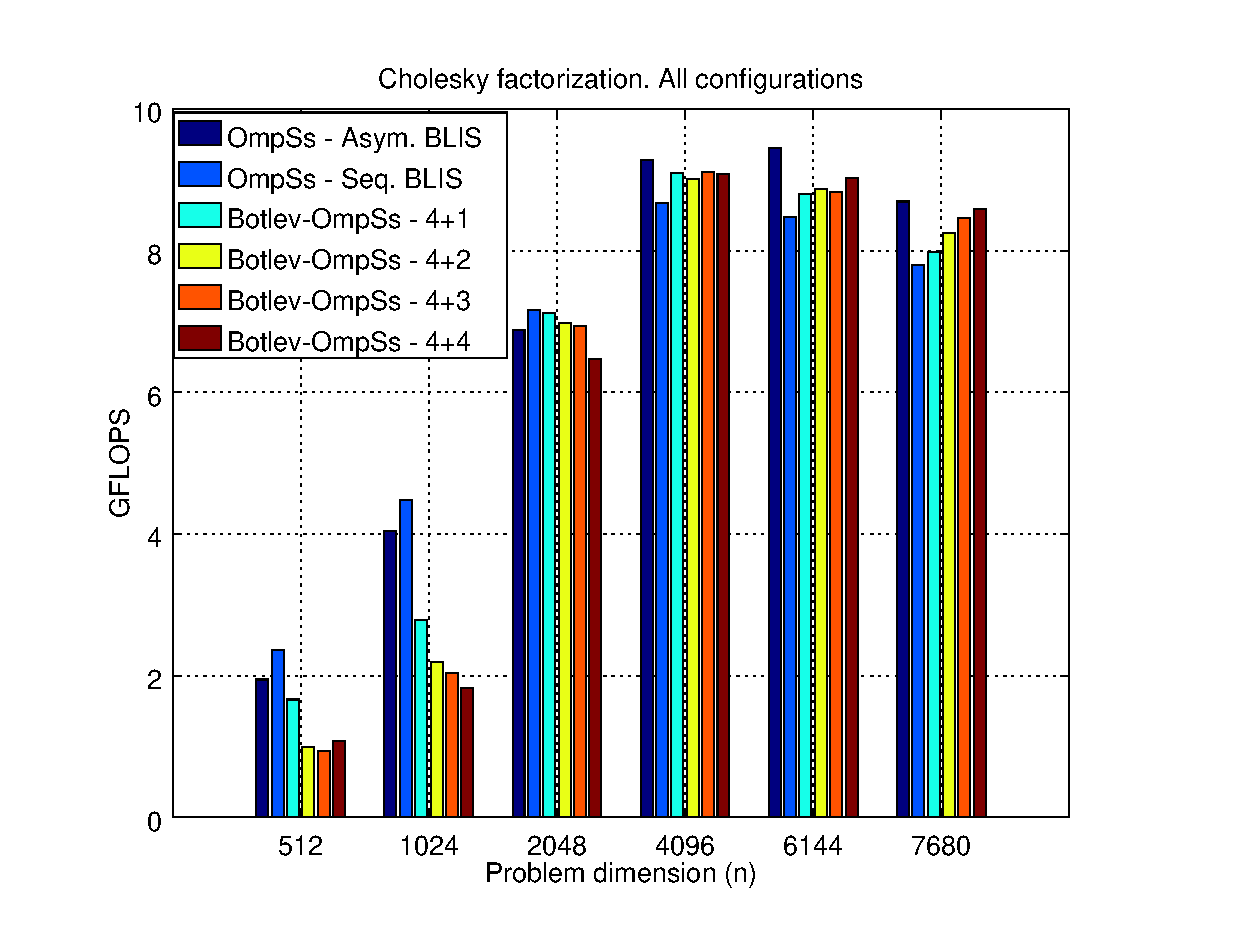
\includegraphics[width=0.70\textwidth]{Plots/Comparative/comparative}
\caption{Rendimiento (en GFLOPS) para la factorización de Cholesky utilizando 
el planificador convencional de OmpSs enlazado con la versión secuencial de BLIS, la implementación asimétrica de BLIS, y 
la implementación consciente de la arquitectura Botlev de OmpSs enlazado con la versión secuencial de BLIS sobre \odroid. 
Las etiquetas con la forma ``4+x'' indican una ejecución con 4~núcleos Cortex-A15 utilizando x núcleos Cortex-A7.}
\label{fig:comparative}
\end{figure}

En conclusión, nuestro enfoque para explotar la asimetría mejora tanto la portabilidad como la facilidad de
programación y desarrollo de planificadores de tareas, evitando el desarrollo de políticas específicas de planificación
conscientes de la asimetría. Además, el rendimiento obtenido es comparable con éstos para cualquier tamaño de problema; para
matrices de tamaño medio/grande, mejora además de forma sustancial el rendimiento conseguido por un planificador no consciente de la
asimetría.

\subsection{Análisis detallado de rendimiento}

A continuación, se proporcionan más detalles sobre el comportamiento, en términos de rendimiento, de cada una de las 
configuraciones anteriormente descritas. Las trazas de ejecución mostradas en esta sección han sido extraídas con la
herramienta de instrumentación {\tt Extrae}~\cite{Extrae} y visualizadas a través de la herramienta {\tt Paraver}~\cite{Paraver}.
Los resultados corresponden a un caso concreto de la factorización de Cholesky, con matriz de entrada de dimensión
{\tt n}~=~6,144 y tamaño de bloque {\tt b}~=~448.

\subsubsection{Visión general de la ejecución de tareas}

La Figura~\ref{fig:traces_tasks} muestra una traza completa de ejecución para cada configuración del planificador OmpSs. A grandes rasgos, es posible
extraer un conjunto de observaciones generales:

\begin{itemize}
\item Desde el punto de vista del tiempo total de ejecución, el planificador convencional de OmpSs combinado con una versión asimétrica
	de BLIS obtiene los mejores resultados, seguido por la implementación Botlev del planificador. Es necesario destacar que
		la versión no consciente de la asimetría de OmpSs, con 8 \wt y sin ninguna modificación adicional, obtiene los peores
		resultados con diferencia. En este caso, el desequilibrio de carga y los largos periodos de inactividad en la
		ejecución de tareas, especialmente a medida que el paralelismo de tareas disponible disminuye (en las últimas etapas
		de la ejecución) conllevan una penalización de rendimiento muy considerable.

\item Las marcas de inicio/finalización de cada tarea revelan que la versión asimétrica de BLIS (que utiliza los recursos combinados
	en cada VC) requiere menor tiempo de ejecución por tarea que las dos alternativas basadas en BLIS secuencial. Un efecto a observar
		es la lógica diferencia en rendimiento en la versión Botlev del planificador en la ejecución de las tareas sobre núcleos
		rápidos (\wts entre el 5 y el 8) y lentos (\wts entre el 1 y el 4). Este fenómeno no se observa en nuestra solución, ya
		que, para el planificador, cualquiera de los 4 \wts disponibles observa unidades de procesamiento (VCs) homogéneos.

\item El planificador Botlev-OmpSs incluye políticas complejas de planificación que incluyen el tratamiento de prioridades,
	avanzando la ejecución de tareas en el camino cŕitico y, cuando sea posible, asignando éstas a núcleos rápidos (véanse,
		por ejemplo, las tareas correspondientes a factorizaciones de los bloques diagonales, coloreadas en amarillo). Esta
		política induce una planificación más compactadurante las primeras fases de la ejecución paralela, pero 
		con mayores problemas a medida que el grado de concurrencia disminuye (en las últimas iteraciones de la 
		factorización). Aunque es posible, no se ha activado este tipo de gestión de prioridades en la versión convencional
		de OmpSs utilizada en el resto de experimentos, y su interacción con una implementación asimétrica de las tareas
		se plantea como trabajo futuro.
\end{itemize}


\begin{figure}%[t]
\centering
	\begin{subfigure}{\textwidth}
   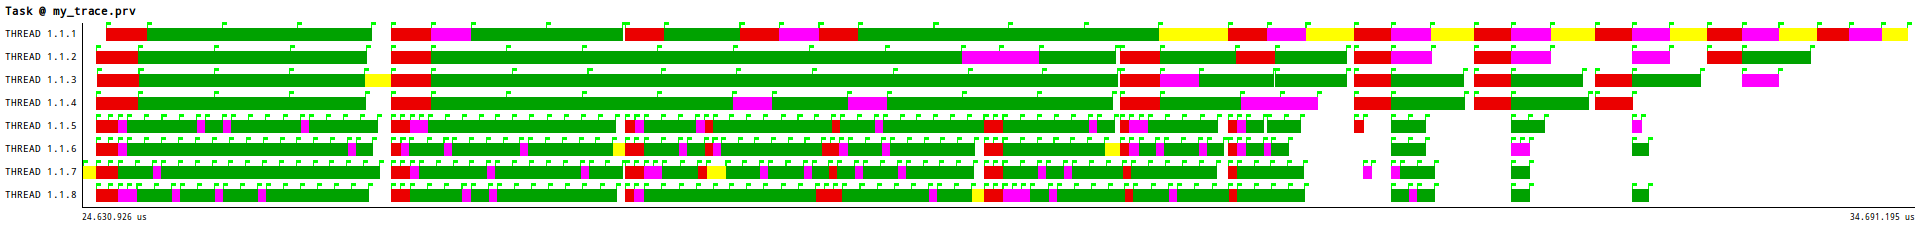
\includegraphics[width=\textwidth]{Plots/Traces/sym_8cores_tasks.png}
		\caption{OmpSs - BLIS secuencial (8 worker threads)} 
	\end{subfigure}
	\begin{subfigure}{\textwidth}
   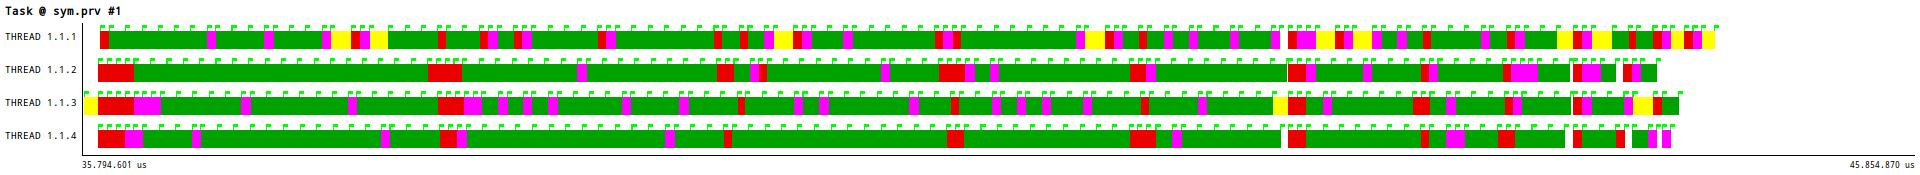
\includegraphics[width=\textwidth]{Plots/Traces/sym_tasks.png}
 \caption{OmpSs - BLIS secuencial (4 worker threads)} 
	\end{subfigure}
	\begin{subfigure}{\textwidth}
   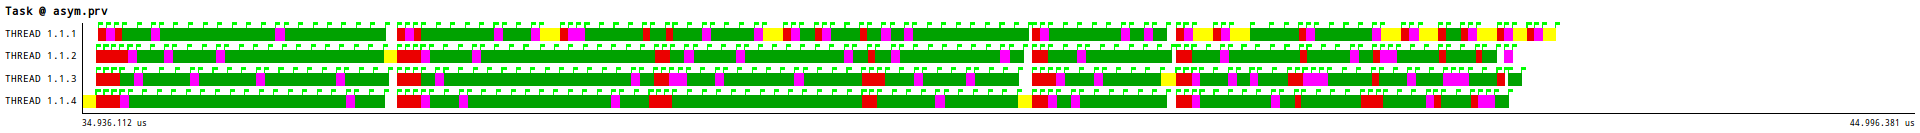
\includegraphics[width=\textwidth]{Plots/Traces/asym_tasks.png}
		\caption{OmpSs - BLIS asimétrico (4 worker threads)}
	\end{subfigure}
	\begin{subfigure}{\textwidth}
   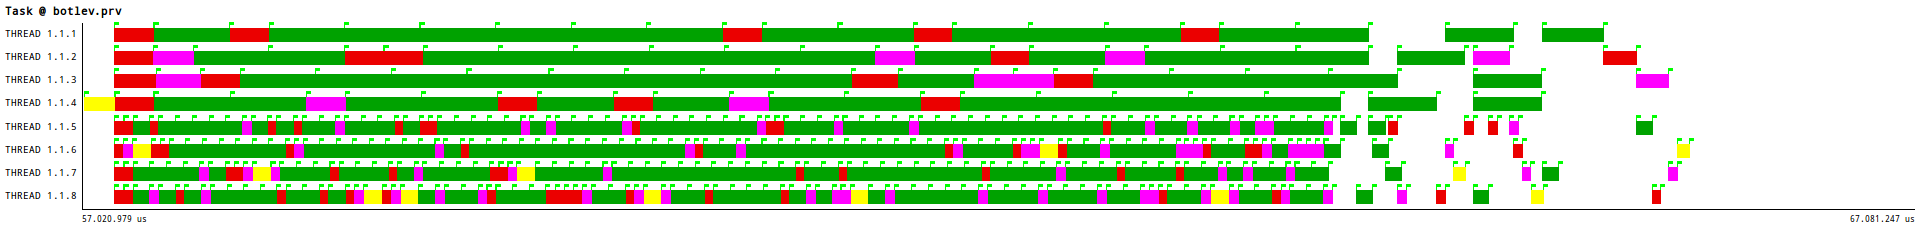
\includegraphics[width=\textwidth]{Plots/Traces/botlev_tasks.png}
		\caption{Botlev-OmpSs - BLIS secuencial (8 worker threads, 4+4)}
	\end{subfigure}
\caption{Trazas de ejecución para las tres configuraciones estudiadas en la factorización de Cholesky ({\tt n}~=~6,144, 
{\tt b}~=~448). 
La línea de tiempo en cada fila recoge las tareas ejecutadas por un único \wt.
Las tareas se han coloreado siguiendo la convención de la Figura~\ref{fig:dag};
las fases coloreadas en color blanco representan etapas sin actividad. Las marcas en color
	verde denotan puntos de inicialización de la ejecución de cada tarea.
}
\label{fig:traces_tasks}
\end{figure}


Se proporciona a continuación un análisis cuantitativo de la duración temporal de las tareas y un estudio
más detallado de la estrategia de planificación integrada en cada configuración.

\subsubsection{Duración de las tareas}
 
La Tabla~\ref{tab:2dp_tasks} muestra el tiempo medio de ejecución por tipo de tarea para cada \wt.
Los resultados muestran como el tiempo de ejecución para cada tipo de tarea es considerablemente menor
en la versión asimétrica de BLIS que en las alternativas basadas en ejecuciones secuenciales de las
tareas. La única excepción es la factorización de los bloques diagonales (rutina {\tt dpotrf}), ya que
se trata de una rutina perteneciente a LAPACK, y por tanto no disponible en BLIS y no paralelizada de forma
consciente de la asimetría). Inspeccionando la duración de las tareas en la configuración Botlev-OmpSs, 
se observa una notable diferencia en función del tipo de núcleo sobre el que el planificador mapea las tareas. Por
ejemplo, el tiempo medio de ejecución para {\tt dgemm} varía entre más de 400~ms en un núcleo lento, hasta prácticamente
90~ms en un núcleo rápido. Este comportamiento se reproduce para todos los tipos de tareas.

Para ilustrar más claramente estas observaciones, la Figura~\ref{fig:traces_task_duration} representa un histograma
detallado de los tiempos de ejecución para las distintas instancias de la tarea {\tt dgemm} durante la ejecución
paralela. Cada casilla corresponde al número de tareas con un tiempo de ejecución dado, mientras que las filas corresponden
a cada \wt en ejecución.
Comparando las configuraciones que utilizan planificadores convencionales (trazas (a) y (b)),
existe una clara desviación en el tiempo medio de ejecución hacia mayores rendimientos al utilizar
BLIS asimétrico, esto es, el tiempo medio de ejecución de una tarea es claramente menor en este caso. El histograma para Botlev (traza (c))
muestra dos zonas diferenciadas, que corresponden a tareas ejecutadas sobre núcleos rápidos y núcleos lentos, respectivamente. Nótese que
las tareas ejecutadas sobre núcleos rápidos obtienen el mismo rendimiento que las equivalentes en una configuración convencional
usando BLIS secuencial. Se ha observado un comportamiento similar para el resto de tareas BLAS ejecutadas durante el experimento.

\begin{figure}%[t]
\centering
	\begin{subfigure}{\textwidth}
   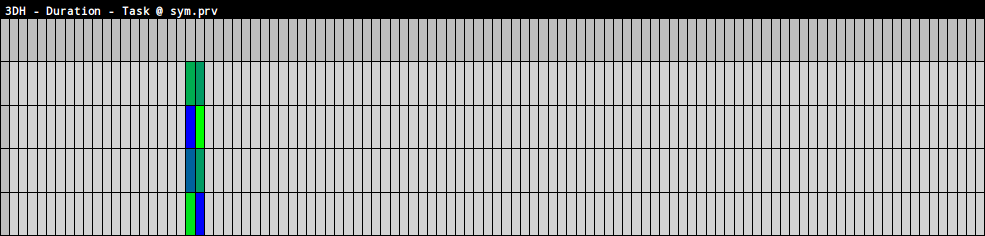
\includegraphics[width=\textwidth]{Plots/Traces/sym_task_duration_histogram.png}
 \caption{OmpSs + Symmetric BLIS}
	\end{subfigure}
	\begin{subfigure}{\textwidth}
   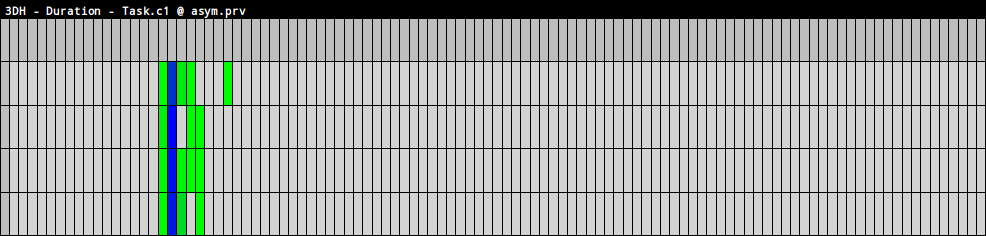
\includegraphics[width=\textwidth]{Plots/Traces/asym_task_duration_histogram.png}
		\caption{OmpSs + Asymmetric BLIS}
	\end{subfigure}
	\begin{subfigure}{\textwidth}
   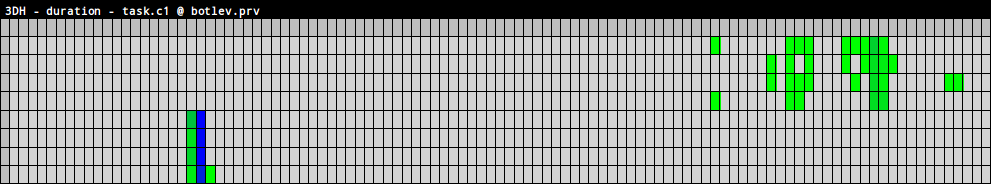
\includegraphics[width=\textwidth]{Plots/Traces/botlev_task_duration_histogram.png}
 \caption{Botlev-OmpSs - 4+4 threads}
	\end{subfigure}
\caption{Histograma de duración de tareas para la tarea {\tt dgemm} sobre las tres configuraciones de planificador utilizadas para la factorización de Cholesky ({\tt n}~=~6,144, {\tt b}~=~448).  
	Las filas corresponden a los \wts en ejecución. Las columnas corresponden a intervalos de tiempo de ejecución medio. Los colores (en gradiente) indican el número de tareas en el 
	intervalo correspondiente (desde verde claro hasta azul oscuro, en un rango de menor a mayor número de tareas).}
\label{fig:traces_task_duration}
\end{figure}


\begin{table}%[t]
\centering
\caption{Average time (in ms) per task and worker thread in the Cholesky factorization  ({\tt n}~=~6,144, 
{\tt b}~=~448), for the three runtime configurations.}
\label{tab:2dp_tasks}

\ra{1.2}
\ca{2pt}

\renewcommand{\fg}[1]{{#1}} 
\renewcommand{\br}[1]{{#1}} 

{\scriptsize
\begin{tabular}{crrrrrrrrrrrrrrr} 
   	\toprule
                 & \phantom{a} & \multicolumn{4}{c}{OmpSs - Seq. BLIS} & \phantom{ab} & \multicolumn{4}{c}{OmpSs - Asym. BLIS} & \phantom{ab} & \multicolumn{4}{c}{Botlev-OmpSs - Seq. BLIS} \\ 
                 & \phantom{a} & \multicolumn{4}{c}{(4 worker threads)} & \phantom{ab} & \multicolumn{4}{c}{(4 worker threads)} & \phantom{ab} & \multicolumn{4}{c}{(8 worker threads, 4+4)} \\ 
                                          \cmidrule{3-6}                                         \cmidrule{8-11}                                      \cmidrule{13-16}
                       & \phantom{a} &    {\tt dgemm} & {\tt dtrsm}& {\tt dsyrk}& {\tt dpotrf}  & \phantom{ab} & {\tt dgemm}  & {\tt dtrsm} & {\tt dsyrk} & {\tt dpotrf}& \phantom{ab} & {\tt dgemm} & {\tt dtrsm} & {\tt dsyrk} & {\tt dpotrf}         \\ \hline 
	 {\sc wt 0}    & \phantom{a} &    \br{89.62} & \fg{48.12} & \fg{47.14} & \fg{101.77}    & \phantom{ab} & \fg{79.82}  & \fg{42.77}  & \fg{44.42}  & \fg{105.77}  & \phantom{ab} & \fg{406.25} & \fg{216.70} & \fg{--} & \fg{--}    \\ \cline{3-16}
	 {\sc wt 1}    & \phantom{a} &    \br{88.96} & \br{48.10} & \fg{47.14} & \fg{--}      & \phantom{ab} & \fg{78.65}  & \fg{42.97}  & \fg{44.56}  & \fg{76.35}  & \phantom{ab} & \fg{408.90} & \fg{207.41} & \fg{212.55} & \fg{--}    \\ \cline{3-16}
	 {\sc wt 2}    & \phantom{a} &    \br{89.02} & \br{48.36} & \br{47.18} & \fg{87.22}    & \phantom{ab} & \fg{79.14}  & \fg{43.14}  & \fg{44.60}  & \fg{85.98}  & \phantom{ab} & \fg{415.31} & \fg{230.07} & \fg{212.56} & \fg{--}    \\ \cline{3-16}
	 {\sc wt 3}    & \phantom{a} &    \br{90.11} & \br{48.51} & \br{47.42} & \fg{--}      & \phantom{ab} & \fg{79.28}  & \fg{43.10}  & \fg{44.59}  & \fg{67.73}  & \phantom{ab} & \fg{410.84} & \fg{216.95} & \fg{216.82} & \fg{137.65}    \\ \cline{3-16}
	 {\sc wt 4}    & \phantom{a} &    \br{--} & \br{--} & \br{--} & \fg{--} & \phantom{ab} & \fg{--}  & \fg{--} & \fg{--} & \fg{--} & \phantom{ab} & \fg{90.97} & \fg{48.97} & \fg{48.36} & \fg{--}    \\ \cline{3-16}
	 {\sc wt 5}    & \phantom{a} &    \br{--} & \br{--} & \br{--} & \fg{--} & \phantom{ab} & \fg{--}  & \fg{--} & \fg{--} & \fg{--} & \phantom{ab} & \fg{90.61} & \fg{48.86} & \fg{48.16} & \fg{90.78}    \\ \cline{3-16}
	 {\sc wt 6}    & \phantom{a} &    \br{--} & \br{--} & \br{--} & \fg{--} & \phantom{ab} & \fg{--}  & \fg{--} & \fg{--} & \fg{--} & \phantom{ab} & \fg{91.28} & \fg{49.43} & \fg{47.97} & \fg{89.58}    \\ \cline{3-16}
	 {\sc wt 7}    & \phantom{a} &    \br{--} & \br{--} & \br{--} & \fg{--} & \phantom{ab} & \fg{--}  & \fg{--} & \fg{--} & \fg{--} & \phantom{ab} & \fg{91.60} & \fg{49.49} & \fg{48.62} & \fg{95.43}    \\ \bottomrule
	 %{\sc TOTAL}   & \phantom{a} &    \br{25.57} & \br{3.76} & \br{3.68} & \fg{1.24} & \phantom{ab} & \fg{22.65}  & \fg{3.35} & \fg{3.47} & \fg{1.26} & \phantom{ab} & \fg{44.07} & \fg{6.51} & \fg{6.12} & \fg{3.14}    \\ \bottomrule
	 {\sc Avg.}     & \phantom{a} &    \br{89.43} & \br{48.27} & \br{47.22} & \fg{94.49} & \phantom{ab} & \fg{79.22}   & \fg{42.99} & \fg{44.54} & \fg{83.96} & \phantom{ab} & \fg{250.72} & \fg{133.49} & \fg{119.29} & \fg{103.36}    \\ \bottomrule
\end{tabular}
}

\end{table}

\subsubsection{Políticas de planificación y tiempos sin actividad}


La Figura~\ref{fig:traces_task_number} ilustra el orden de ejecución de tareas determinado por el planificador de OmpSs. 
En ella, las tareas se muestran utilizando un gradiente de color, atendiendo exclusivamente al orden en el que son encontradas
en el código secuencial (Figura~\ref{lst:chol}), desde la primera hasta la última.

En tiempo de ejecución, el planificador de tareas Botlev-OmpSs lanza tareas a ejecución fuera de orden, dependiendo de
su criticalidad, y las asigna, a ser posible, sobre núcleos rápidos. De acuerdo con esta estrategia, la ejecución fuera de
orden se revela más frecuentemente en las líneas de tiempo para los núcleos rápidos que para los lentos. Con el planificador
convencional, la ejecución fuera de orden sólo viene dictada por el cumplimiento de las dependencias de datos en tiempo de ejecución.

A la vista de las trazas de ejecución, es posible observar cómo el planificador Botlev-OmpSs muestra una penalización
en el rendimiento muy apreciable debida a la existencia de periodos ociosos en la parte final de la factorización, cuando
la concurrencia disponible disminuye. Este problema no se da utilizando políticas de planificación convencionales. Sin embargo,
en las primeras fases de la factorización, el uso de una política consciente de la criticalidad de las tareas (implementada en 
Botlev-OmpSs), reduce de forma efectiva los períodos de tiempo en los que los \wts permanecen ociosos.

La Tabla~\ref{tab:th_state} muestra el porcentaje de tiempo en el que cada \wt permanece en estado 
{\tt running} (ejecutando tareas) o {\tt idle} (sin ejecutar tareas). En general, la cantidad de tiempo transcurrido en estado
{\tt idle} es mucho mayor para Botlev-OmpSs que para las implementaciones convencionales
(17\% contra 5\%, respectivamente). 
Nótese también la notable diferencia en el porcentaje de tiempo ocioso entre núcleos rápidos y lentos
(20\% y~13\%, respectivamente), lo que lleva a la conclusión de que los núcleos rápidos deben esperar 
a la finalización de tareas ejecutadas en núcleos lentos. En otras palabras, en estas configuraciones, los núcleos lentos ``frenan'' a los
rápidos. Este hecho es también constatable en las etapas finales de la traza obtenida con la configuración Botlev-OmpSs.

Las anteriores observaciones sugieren la combinación de distintas configuraciones sobre una misma ejecución si
se utilizan procesadores asimétricos; en este enfoque, la asimetría podría ser explotada a través de políticas de planificación
conscientes de la arquitectura durante las primeras fases de la factorización --cuando el paralelismo de tareas disponible es elevado--,
y reemplazar el enfoque por el uso de tareas conscientes de la arquitectura y VCs en las fases finales de la ejecución, cuando la
concurrencia es escasa. Ambos enfoques no son mutuamente exclusivos, sino complementarios en función del nivel de concurrencia disponible
en un punto determinado de la ejecución. Estas ideas se plantean como líneas de investigación futuras al presente trabajo.

\begin{figure}%[t]
\centering
	\begin{subfigure}{\textwidth}
   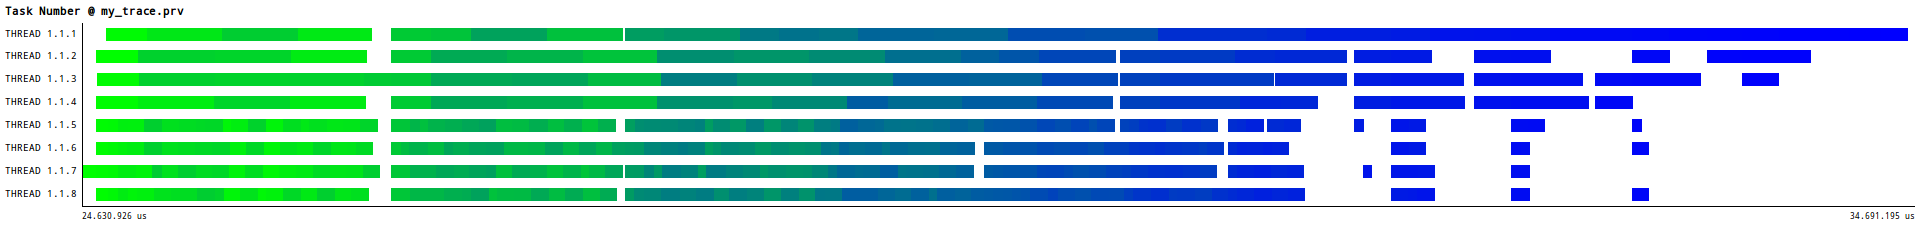
\includegraphics[width=\textwidth]{Plots/Traces/sym_8cores_task_number.png}
		\caption{OmpSs - BLIS secuencial (8 worker threads)}
	\end{subfigure}
	\begin{subfigure}{\textwidth}
   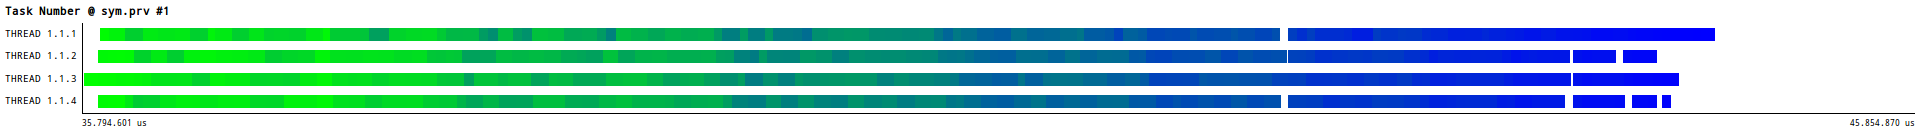
\includegraphics[width=\textwidth]{Plots/Traces/sym_task_number.png}
		\caption{OmpSs - BLIS secuencial (4 worker threads)} 
	\end{subfigure}
	\begin{subfigure}{\textwidth}
   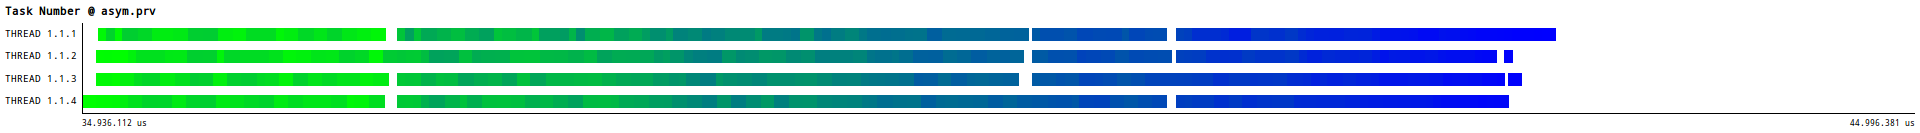
\includegraphics[width=\textwidth]{Plots/Traces/asym_task_number.png}
		\caption{OmpSs - BLIS asimétrico (4 worker threads)} 
	\end{subfigure}
	\begin{subfigure}{\textwidth}
   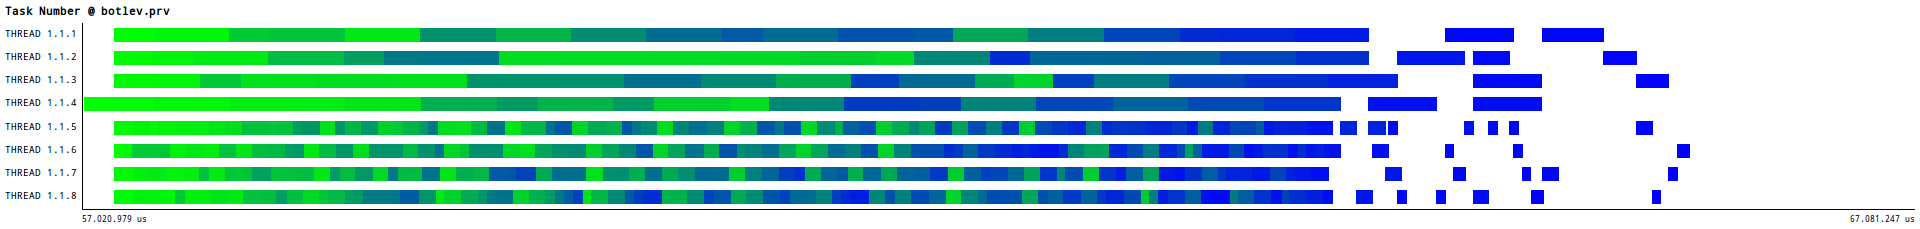
\includegraphics[width=\textwidth]{Plots/Traces/botlev_task_number.png}
		\caption{Botlev-OmpSs - BLIS secuencial (8 worker threads, 4+4)} 
	\end{subfigure}
\caption{Orden de ejecución de tareas para las tres configuraciones estudiadas sobre la factorización de Cholesky
({\tt n}~=~6,144, {\tt b}~=~448). En las trazas, las tareas se ordenan según su orden de aparición
en el código secuencial, y son mostradas usando un gradiente de color, correspondiendo el color verde claro a tareas
	tempranas, y azul oscuro a tareas tardías.}
\label{fig:traces_task_number}
\end{figure}

\begin{table}
\centering
	\caption{Porcentaje de tiempo por \wt en estado {\tt idle} o {\tt running} para distintas configuraciones de planificador para la factorización de Cholesky
({\tt n}~=~6,144, {\tt b}~=~448).
	Nótese que {\sc wt 0} es el hilo principal, y por tanto nunca permanece en estado {\tt idle} dadas las características de OmpSs; 
	para él, el resto del tiempo hasta el 100\% se dedica a sincronización, planificación y creación de la hebra. Para el resto de las hebras, esta cantidad
	de tiempo se considera sobrecoste de planificación ({\tt runtime overhead}).}
\label{tab:th_state}

\ra{1.2}
\ca{2pt}

\renewcommand{\fg}[1]{{#1}} 
\renewcommand{\br}[1]{{#1}} 

{\scriptsize
\begin{tabular}{crrrrrrrrr} 
   	\toprule
                 & \phantom{a} & \multicolumn{2}{c}{OmpSs - Seq. BLIS} & \phantom{ab} & \multicolumn{2}{c}{OmpSs - Asym. BLIS} & \phantom{ab} & \multicolumn{2}{c}{Botlev-OmpSs - Seq. BLIS} \\ 
                 & \phantom{a} & \multicolumn{2}{c}{(4 worker threads)} & \phantom{ab} & \multicolumn{2}{c}{(4 worker threads)} & \phantom{ab} & \multicolumn{2}{c}{(8 worker threads, 4+4)} \\ 
                 %& \phantom{a} & \multicolumn{4}{c}{OmpSs - Seq. BLIS} & \phantom{ab} & \multicolumn{4}{c}{OmpSs - Asym. BLIS} & \phantom{ab} & \multicolumn{4}{c}{Botlev-OmpSs - Seq. BLIS} \\ 
                 %& \phantom{a} & \multicolumn{4}{c}{(4 worker threads)} & \phantom{ab} & \multicolumn{4}{c}{(4 worker threads)} & \phantom{ab} & \multicolumn{4}{c}{(8 worker threads, 4+4)} \\ 
                                          \cmidrule{3-4}                                         \cmidrule{6-7}                                      \cmidrule{9-10}
                       & \phantom{a} &    {\tt idle}& {\tt running}& \phantom{ab}  & {\tt idle}& {\tt running}& \phantom{ab} & {\tt idle}  & {\tt running} \\ \hline 
	 {\sc wt 0}    & \phantom{a} &    \fg{--}   & \fg{98.41}   & \phantom{ab}  & \fg{--}   & \fg{97.85}   & \phantom{ab} & \fg{--}     & \fg{86.53}    \\ \cline{3-10}
	 {\sc wt 1}    & \phantom{a} &    \br{5.59} & \fg{94.22}   & \phantom{ab}  & \fg{5.51} & \fg{94.29}   & \phantom{ab} & \fg{13.63}  & \fg{86.28}    \\ \cline{3-10}
	 {\sc wt 2}    & \phantom{a} &    \br{3.14} & \fg{96.67}   & \phantom{ab}  & \fg{5.27} & \fg{94.53}   & \phantom{ab} & \fg{13.94}  & \fg{85.98}    \\ \cline{3-10}
	 {\sc wt 3}    & \phantom{a} &    \br{5.77} & \fg{94.07}   & \phantom{ab}  & \fg{5.17} & \fg{94.62}   & \phantom{ab} & \fg{13.43}  & \fg{86.47}    \\ \cline{3-10}
	 {\sc wt 4}    & \phantom{a} &    \br{--}   & \fg{--}      & \phantom{ab}  & \fg{--}   & \fg{--}      & \phantom{ab} & \fg{19.26}  & \fg{80.51}    \\ \cline{3-10}
	 {\sc wt 5}    & \phantom{a} &    \br{--}   & \fg{--}      & \phantom{ab}  & \fg{--}   & \fg{--}      & \phantom{ab} & \fg{21.12}  & \fg{78.69}    \\ \cline{3-10}
	 {\sc wt 6}    & \phantom{a} &    \br{--}   & \fg{--}      & \phantom{ab}  & \fg{--}   & \fg{--}      & \phantom{ab} & \fg{20.84}  & \fg{78.97}    \\ \cline{3-10}
	 {\sc wt 7}    & \phantom{a} &    \br{--}   & \fg{--}      & \phantom{ab}  & \fg{--}   & \fg{--}      & \phantom{ab} & \fg{20.09}  & \fg{79.70}    \\ \bottomrule
	 %{\sc TOTAL}   & \phantom{a} &    \br{13.87} & \fg{384.31}    & \phantom{ab}  & \fg{16.97}  & \fg{379.60}    & \phantom{ab} & \fg{73.81}  & \fg{715.16}   \\ \bottomrule
	 {\sc Avg.}     & \phantom{a} &    \br{4.84} & \fg{95.89}    & \phantom{ab} & \fg{5.32} & \fg{94.90}   & \phantom{ab} & \fg{17.47}  & \fg{82.89}    \\ \bottomrule
\end{tabular}
}

\end{table}



%-- Configuraciones para emacs --
%%% Local Variables:
%%% mode: latex
%%% TeX-master: "./principal.tex"
%%% End:

\cleardoublepage

\chapter{Optimización de la eficiencia energética de OmpSs sobre arquitecturas asimétricas}
\label{ch:chapter5}

\section{Descripción de la estrategia de optimización}

\subsection{DVFS sobre la arquitectura big.LITTLE}

\subsection{Evaluación de rendimiento/eficiencia energética de las tareas}


\section{Políticas de reducción de consumo}

\subsection{P1}
%%
\comentario{Reescribir}%%
Durante la ejecución de un programa paralelo mediante un paradigma basado
en tareas, puede ocurrir el caso en el que la mayor parte de tareas listas
para ser ejecutadas sean críticas, provocando que no existan más tareas
listas hasta que estas acaben. Un ejemplo de aplicación con este
comportamiento sería aquella cuyo árbol de dependencias se encogiera muy
rápidamente en algún punto intermedio de la ejecución, para luego volverse
a expandir rápidamente (un árbol con forma de diábolo). En este árbol, las
tareas del cuello de botella del medio serían tareas críticas ya que son
prioritarias para que la ejecución continúe su ejecución, y además, en el
momento que esto ocurra, un gran número de tareas estarán listas para ser
ejecutadas y
poder continuar la ejecución del problema.\\
Este problema aplicado al planificador botlev supondría que en el momento
en el que el árbol se estreche, la cola de tareas no críticas tendría un
tamaño mucho inferior al de tareas críticas, y por tanto los cores LITTLE
tendrían mucha menor carga de trabajo que los cores big. Esto ocurriría
mientras que los cores big finalicen la ejecución de sus tareas críticas y
se preparen más tareas para ejecutar por los cores LITTLE.\\
Aunque una forma de intentar paliar este problema sería obligar a que los
cores lentos ejecutaran tareas críticas, esto podría provocar que se
retrase la finalización de una tarea crítica, ya que aunque su ejecución
puede comenzar antes (pues se disponen de más cores para distribuir el
mismo número de tareas), el rendimiento de los cores LITTLE es mucho
inferior que el de los cores big, provocando retrasos en la ejecución,
incluso llegando a aumentar el problema del cuello de botella.

La política P1 intenta reducir este problema desde un enfoque distinto. La
idea principal que se encuentra detrás de esta política es la de aprovechar
estos momentos en los que la carga de trabajo sobre los cores lentos es
menor para intentar disminuir el consumo energético aplicando una reducción
de frecuencia sobre el cluster LITTLE. Como se podía ver en la
figura~\todo{ref}, reducir la frecuencia al cluster LITTLE implica que la
potencia instantánea disminuye. Es cierto que al reducir la frecuencia de
los cores el tiempo usado en ejecutar una tarea aumenta, pero como esta
técnica únicamente se aplica en los momentos en los que la ejecución está
limitada por el gran número de tareas críticas y el bajo número de tareas
no críticas, se espera que el impacto final en el rendimiento no sea muy
elevado.\\
La forma de aplicar esta política sobre botlev consiste en monitorizar
constantemente el número de tareas tanto críticas como no críticas listas
para ser ejecutadas (reflejado en el tamaño de las colas internas del
planificador), y actuar en función a la relación entre el tamaño de ambas
colas. La figura~\ref{s5:fig:listing-p1} muestra un fragmento esquemático
del código encargado de realizar esta tarea. Este método es invocado cada
vez que el tamaño de una cola cambia (ya sea porque una tarea comienza su
ejecución, o porque una tarea se encuentra lista para ser ejecutada y es
introducida en una cola). Como se puede ver en la
línea~\ref{s5:lst:p1-calculoPrincipal(a)}, la frecuencia a la que cambiar
el cluster se calcula como una proporción directa entre el tamaño de ambas
colas, así, si el número de tareas críticas es el doble que el de las
tareas no críticas, la frecuencia se disminuye un escalón; si el tamaño es
el triple, la frecuencia se disminuye hasta el tercer escalón de
frecuencia, etc. Recordar que los valores de frecuencia que puede tomar el
cluster están limitados por el kernel del sistema operativo, como se
mencionó en la sección~\todo{ref}. La
línea~\ref{s5:lst:p1-calculoPrincipal(b)} asegura que la frecuencia final
no es menor que la menor frecuencia soportada. Destacar que de esta manera
se consigue que el cambio de frecuencia en el cluster se realice de manera
escalonada según varía el tamaño de las colas.\\
%%%
\comentario{La línea 8 es un poco desconcertante}
%%%
\begin{figure}
  \centering

  \begin{lstlisting}[language=C++]
int P1(int bigQueueSize, int littleQueueSize){
  int nxtFreq;
      
  if( littleQueueSize==0 ) nxtFreq = FreqCfg::minLittleFreq; |\label{s5:lst:p1-casoEsp1}|
  else if( bigQueueSize==0 ) nxtFreq = FreqCfg::maxLittleFreq; |\label{s5:lst:p1-casoEsp2}|
  else{
    int idx = min((bigQueueSize / littleQueueSize), |\label{s5:lst:p1-calculoPrincipal(a)}|
                   FreqCfg::maxIdxLittle );         |\label{s5:lst:p1-calculoPrincipal(b)}|
    nxtFreq = FreqCfg::littleFreqs[idx];
  }
  return changeLittleFreq(nxtFreq);
}
\end{lstlisting}

  \caption[Fragmento de código esquemático para la política P1]
  {Fragmento de código esquemático para la política P1.}
  \label{s5:fig:listing-p1}
\end{figure}

Adicionalmente al comportamiento general de esta política, hay que
distinguir dos casos especiales que merecen ser mencionados: el caso en el
que no exista ninguna tarea crítica lista para ser ejecutada, y el caso
opuesto en el que todas las tareas listas sean críticas y los cores lentos
estén totalmente ociosos. En estos casos, las
líneas~\ref{s5:lst:p1-casoEsp1}-\ref{s5:lst:p1-casoEsp2} se encargan de
aumentar la frecuencia al máximo directamente en caso de que todas las
tareas sean no críticas, o de disminuir la frecuencia al mínimo en caso de
que no exista ninguna tarea no crítica que ejecutar.

\todo{quizás poner aquí la evolución de la frecuencia en funcińo del tamaño
  de las colas. Puede que mejor en la sección de resultados}.

\subsection{P2 y P2'}
A la hora de aplicar técnicas de escalado de frecuencia (DVFS) sobre una
arquitectura o problema, la técnica presenta de manera simplificada dos
grandes dimensiones sobre las que tomar decisiones sobre los parámetros de
configuración para conseguir el objetivo de reducir el consumo total:
(a)~una primera dimensión que determina qué frecuencias utilizar durante
los diferentes cambios, y (b)~una segunda dimensión que determina en qué
momentos de la ejecución se debe modificar la frecuencia.\\
La primera dimensión normalmente viene acotada por la propia arquitectura
sobre la que se ejecuta el problema, ya que es común que el procesador no
pueda funcionar a cualquier frecuencia, sino solamente a una serie de
frecuencias prefijadas de antemano. Esto hace que tomar la decisión de a
qué frecuencia se desea cambiar el procesador sea únicamente realizar una
elección en un conjunto cerrado y finito de frecuencias. Destacar que en
ocasiones puede ser interesante descartar algunas de estas frecuencias y no
tenerlas en consideración, ya sea porque impactan de manera muy negativa en
el rendimiento, o no tienen un impacto muy significativo en la mejora de
consumo.\\
La segunda dimensión está estrechamente relacionada con el problema a
ejecutar y el conocimiento que se tenga de él. Las decisiones que se pueden
tomar van desde decisiones de grano grueso, como puede ser tener en cuenta
el nivel de carga de trabajo de cada procesador y variar la frecuencia en
función de este dato, hasta decisiones de grano más fino como puede ser
conocer el comportamiento de cada una de las tareas a ejecutar y el árbol
de dependencias de antemano, y tomar decisiones en función de estos
parámetros, por ejemplo, si se sabe que una tarea es crítica, aumentar la
frecuencia para así intentar generar nuevas tareas cuanto antes, o si se
sabe que la ejecución va a estar bloqueada hasta que no finalice una tarea
en concreto, disminuir la frecuencia del resto de procesadores hasta que
esta tarea finalice y así intentar disminuir el consumo energético. Hay que
hacer notar que aunque bajar la frecuencia del procesador implique
conseguir una potencia instantánea menor, eso no implica que la energía
final consumida sea también menor, ya que al bajar la frecuencia el tiempo
de ejecución puede aumentar lo suficiente provocando un consumo de energía
mayor al final.\\
Adicionalmente a estas dos dimensiones, los sistemas heterogéneos, y en
concreto las arquitecturas asimétricas, presentan una dimensión extra sobre
la que tomar decisiones: (c) decidir sobre qué elementos de cálculo aplicar
el escalado de frecuencia. En el caso de las arquitecturas asimétricas,
esta decisión se simplifica a decidir si aplicar el escalado al cluster de
cores big, o al cluster de cores LITTLE.\\

La primera intuición que surge al intentar aplicar un escalado de
frecuencia sobre una arquitectura asimétrica es la de pensar que debido a
la gran diferencia de rendimiento entre los cores big y LITTLE (como se
pudo ver en la figura~\todo{ref}), aplicar la técnica a los cores big puede
suponer una pérdida significativa de rendimiento, lo cuál puede provocar
incluso un aumento en el consumo energético al tardar mayor tiempo en
ejecutarse la aplicación, es decir, se podría llegar a empeorar tanto el
rendimiento como el consumo energético. Para evitar que suceda este hecho,
las políticas P2 y P2' han sido diseñadas para modificar la frecuencia
sobre el cluster de cores LITTLE, y así intentar no causar un gran impacto
sobre el rendimiento. Además, las políticas han sido desarrolladas sobre el
planificador botlev comentando en la seccion~\ref{s3:botlev}, con el
objetivo de intentar asegurar que las tareas críticas se ejecutan en los
cores big para así evitar que se retrasen si se ejecutaran en un core
LITTLE con la frecuencia disminuida.\\
Para determina cuando variar la frecuencia del cluster se tienen en cuenta
el número de tareas listas para ser ejecutadas, así, si existen muchas
tareas para ser ejecutadas, la frecuencia será alta para intentar finalizar
la ejecución cuanto antes, mientras que si existen pocas tareas listas para
ser ejecutadas la frecuencia será menor, intentando favorecer el ahorro
energético. Este planteamiento es similar a tener en cuenta la carga de
trabajo del sistema, pero medida en número de tareas pendientes en vez de
ciclos ociosos del procesador. Más concretamente, las políticas monitorizan
el tamaño de la cola de tareas listas para ser ejecutadas, y determinan
cuál es el tamaño máximo de la cola hasta el momento de manera dinámica. Si
la cola posee un tamaño igual o superior al tamaño máximo conocido,
significa que el número de tareas es elevado y por tanto la frecuencia debe
ser elevada. Si el tamaño es menor, entonces se determina en que porcentaje
es menor, y en función de las frecuencias consideradas se toma la decisión
de modificar la frecuencia actual o no. En el código de la
figura~\ref{s5:fig:listing-p2} se muestra el pseudocódigo asociado a estas
políticas. El bloque \texttt{if} de la línea~\ref{s5:lst:p2-detectPico} es
el encargado de determinar si el tamaño actual de la cola es mayor o igual
que cualquier tamaño hasta el momento, y en caso de ser así, configurar el
cluster para que funcione a máxima frecuencia. Esto es equivalente a
determinar si hay un pico de carga de trabajo o no. Las
líneas~\ref{s5:lst:p2-tamStep1}-\ref{s5:lst:p2-tamStep2} determinan el
número de tareas que separan una frecuencia de la otra. La forma de
determinar esta cantidad consiste en repartir de manera equitativa el
espacio máximo de tareas conocido hasta el momento entre todas las
frecuencias, y asignar la frecuencia actual en función de qué tamaño posea
la cola (línea~\ref{s5:lst:p2-step}). Por ejemplo, si el cluster es capaz
de ejecutarse a 5 frecuencias distintas, y hasta el momento el número
máximo de tareas preparadas para ser ejecutas ha sido de 20 tareas, antes
de cambiar de frecuencia se dispone de un margen de 4 tareas. Si el tamaño
actual de la cola es de 3 tareas, la frecuencia del cluster será la mínima,
mientras que si es de 5 tareas, la frecuencia ya no será la mínima, sino la
frecuencia inmeditamente superior.

\begin{figure}
  \centering

  \begin{lstlisting}[language=C++]
int P2(int littleQueueSize, int bigQueueSize){      
  //Comprobamos si estamos en un pico de carga
  if(littleQueueSize >= FreqCfg::maxQueueSize){ |\label{s5:lst:p2-detectPico}|
    FreqCfg::maxQueueSize = littleQueueSize;

    return changeLittleFreq(FreqCfg::maxLittleFreq);
  }

  //Tamanyo para cambiar de frecuencia
  float tamStep = (FreqCfg::maxQueueSize*1.0 /     |\label{s5:lst:p2-tamStep1}|
                   (FreqCfg::maxIdxLittle+1)*1.0); |\label{s5:lst:p2-tamStep2}|
  //Escalon actual
  int step = (int) (littleQueueSize / tamStep);    |\label{s5:lst:p2-step}|

  return changeLittleFreq(FreqCfg::littleFreqs[step]);
}
  \end{lstlisting}

  \caption{Pseudocódigo para las políticas P2 y P2'.}

  \label{s5:fig:listing-p2}
\end{figure}

La diferencia entre las políticas P2 y P2' se encuentra en el rango de
frecuencias que se consideran para el cluster. Así, la política P2 divide
el tamaño de la cola entre todas las frecuencias posibles para el
procesador, mientras que la política P2' solamente considera la frecuencia
máxima y mínima del mismo. 

\begin{figure}
  \centering
  
\includegraphics[width=0.5\textwidth]{Figures/todo.png}

  \caption{Cambios de frecuencia en función del tamaño de las colas para la
    política P2 y P2'.}
  \label{s5:fig:p2}
\end{figure}








\subsection{P3}

\subsection{P4}

\subsection{\ldots}


\section{Resultados experimentales}



%-- Configuraciones para emacs --
%%% Local Variables:
%%% mode: latex
%%% TeX-master: "./principal.tex"
%%% End:

\cleardoublepage

\chapter{Conclusiones}
\label{ch:chapter6}

\section{Conclusiones y trabajo futuro}

En este trabajo se han desarrollado un conjunto de técnicas sobre
arquitecturas asimétricas, y en especial para los procesadores big.LITTLE
diseñados por ARM, que buscan obtener mejoras tanto en el rendimiento de las
aplicaciones como en la eficiencia energética de la plataforma.

En base a un paradigma basado en la extracción de paralelismo a nivel de tareas
en tiempo de ejecución, y 
a través de una versión de la biblioteca BLIS adaptada a arquitecturas asimétricas, 
y basándose en un planificador de tareas convencional, se ha
demostrado como es posible obtener un mejor rendimiento sin necesidad de
adaptar el código del problema a la arquitectura, o introducir cambios
específicos en el planificador. Esta propuesta permite reutilizar los
\emph{runtimes} convencionales (y todas las técnicas desarrolladas durante
los últimos años) sobre las nuevas arquitecturas asimétricas con el único
coste de la implementación de versiones asimétricas de cada tarea.
Los experimentos realizados han demostrado que esta solución es
totalmente comparable con un planificador consciente de la asimetría de la
plataforma, incluso llegando a obtener mejores resultados en el rendimiento
de la aplicación. Esta técnica ha sido presentada en \emph{``The Sixth
  International Workshop on Accelerators and Hybrid Exascale Systems
  (AsHES)''}, a través del artículo~\cite{ashes} mostrado en la
bibliografía.

Buscando la mejora de la eficiencia energética, se han desarrollado una
serie de políticas integradas sobre un planificador consciente de la
asimetría, basadas tanto en técnicas de escalado de frecuencia (DVFS) como
en técnicas de planificación, tomando las decisiones de forma dinámica en
función del número de tareas listas para ser ejecutadas en cada momento. El
primer conjunto de experimentos realizados muestran como,
independientemente de las dos plataformas sobre las que se han ejecutado
los experimentos, aplicar técnicas de escalado de frecuencia sobre el
cluster de núcleos \BIG obtiene una mejora en el rendimiento energético
significativa frente a un planificador convencional consciente de la
asimetría sin ninguna política de ahorro energético integrada.

De igual manera, el segundo conjunto de experimentos revela como en
aquellos procesadores que permiten desactivar un cluster completo a nivel
\emph{hardware}, apagarlo en ciertos momentos de la ejecución cuando el
nivel de tareas listas es lo suficientemente bajo permite obtener una
mejora de rendimiento energético reduciendo la potencia instantánea media
consumida drásticamente. También se ha puesto de manifiesto como, en los
procesadores que no soportan un apagado del cluster a nivel físico, una
política de planificación de tareas que no asigne tareas a ese cluster
obtiene los mismos resultados de eficiencia energética que el planificador
normal consciente de la asimetría.


Como trabajo futuro, se considera realizar los experimentos sobre un
conjunto de problemas de interés científico mayor, así como sobre otras
arquitecturas donde el número de núcleos big y LITTLE se encuentre más
desequilibrado. Adicionalmente, se considera desarrollar políticas que
tomen decisiones de manera dinámica en base al problema ejecutado y su DAG
correspondiente, así como a resultados parciales tomados durante la
ejecución de las distintas tareas previas del problema.



%-- Configuraciones para emacs --
%%% Local Variables:
%%% mode: latex
%%% TeX-master: "./principal.tex"
%%% End:


% +-------------------------------------------------------------------------+
% | References                                                              |
% +-------------------------------------------------------------------------+

% +-------------------------------------------------------------------------+
% | In order for WinEDT to index references correctly, it has to know where |
% | the file resides.  The following command is prefaced by %, and will be  |
% | ignored completely by LaTeX.  However, WinEDT will use this line to     |
% | access the external .bib bibliography file.  Also note that WinEDT can  |
% | read file path names with either "\" or "/" - LaTeX, however, doesn't   |
% | like "\", so it's easier to store a path name in the "Unix" style.      |
% +-------------------------------------------------------------------------+

%Included for Gather Purpose only.  Do NOT uncomment:
%input "references.bib"

% +--------------------------------------------------------------------+
% | This template uses the BibTeX program to format references.  The
% | 3 lines below create a separate Bibliography section and add
% | an entry for "Bibliography" to the Table of Contents.  The actual
% | data for your references (author, title, journal, date, etc.) are
% | entered in the references.bib file.  See that file for information
% | on how to enter references.
% +--------------------------------------------------------------------+

%\bibdata{references}
\bibliographystyle{abbrv}
\bibliography{references,asymmetric,fran,energy}
\addcontentsline{toc}{chapter}{Bibliografía}

% +--------------------------------------------------------------------+
% | Finally, we generate the appendix.  To add or delete appendices,
% | add or remove the line
% |
% |     \input{appendixX.tex}
% |
% | where "X" is the letter designation of the Appendix (A, B, C, etc.)
% | You should have one \input{appendixX.tex} line and a corresponding
% | file appendixX.tex for each appendix.                                 |
% +--------------------------------------------------------------------+

\appendix
\cleardoublepage

\chapter{Anexo}
\label{Appendix1}

%-- Configuraciones para emacs --
%%% Local Variables:
%%% mode: latex
%%% TeX-master: "./principal.tex"
%%% End:


\end{document}
